\begin{comment}
Chapter 5: Results
Results that illustrate how the system designed by you works in practice, and how it is intended to be used, may be presented in this chapter. Screen shots may be useful to illustrate how the software interacts with the user.
\end{comment}

\chapter[Results]{Results}

\section{System Walkthrough}
Below, an overview of the systems behaviour is given following the standard users use case in the form of a walk through. For further exploration of features the application can be found online at \url{https://secure.pezcuckow.com/} where an account can be registered for access.

\begin{figure}
\centering
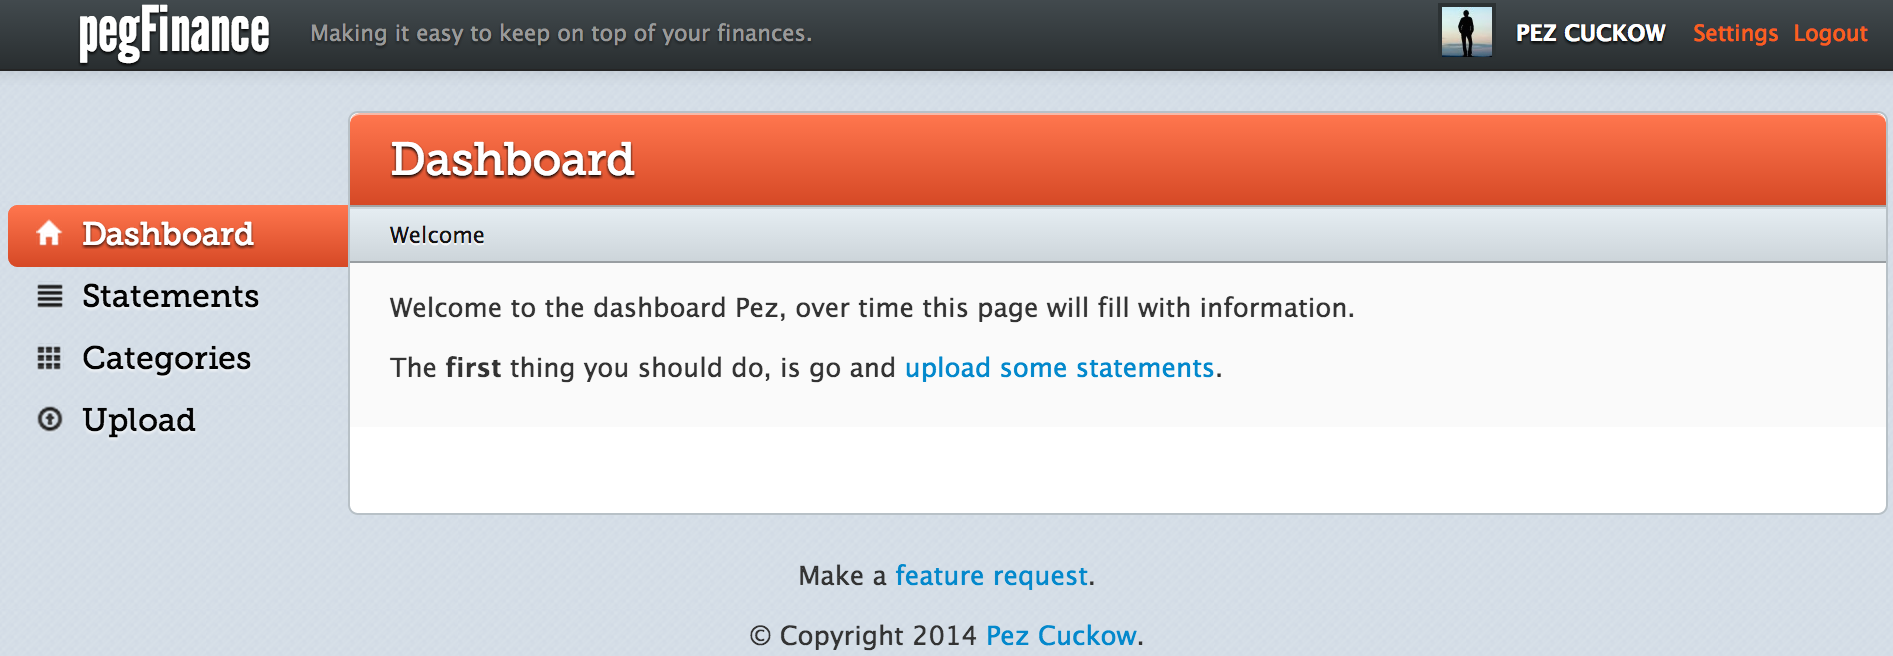
\includegraphics[width=0.8\textwidth]{screenshots/walkthrough/dashboard-empty}
\caption{Empty welcome screen}
\label{fig:welcomescreen}
\end{figure}

Having logged in, the application starts on a welcome screen (Fig. \ref{fig:welcomescreen}) which fills with information over time, for now the system prompts the user to upload a bank statement. The user bar appears at the top of every page\footnote{For clarity both the background and bar are not shown in the following screenshots} which identifies the currently logged in user by name and a avatar pulled using from Gravatar\parencite{gravatar2014avatars}, it provides quick access to the user settings and allows the user to logout.

\begin{figure}
\centering
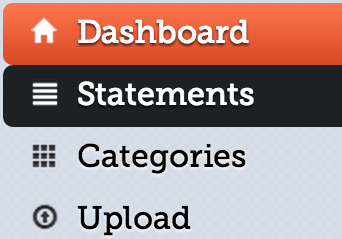
\includegraphics{screenshots/walkthrough/mainmenu}
\caption{Application main menu}
\label{fig:mainmenu}
\end{figure}

On the left hand side of the screen is the main menu (Fig. \ref{fig:mainmenu}), which is also displayed on all pages. It indicated the currently open page in orange, in theme with the rest of the website, and on hover with a mouse it highlights the chosen page by inverting the colors to make the selection clear.

\subsection{Statement Upload}

\begin{figure}
\centering
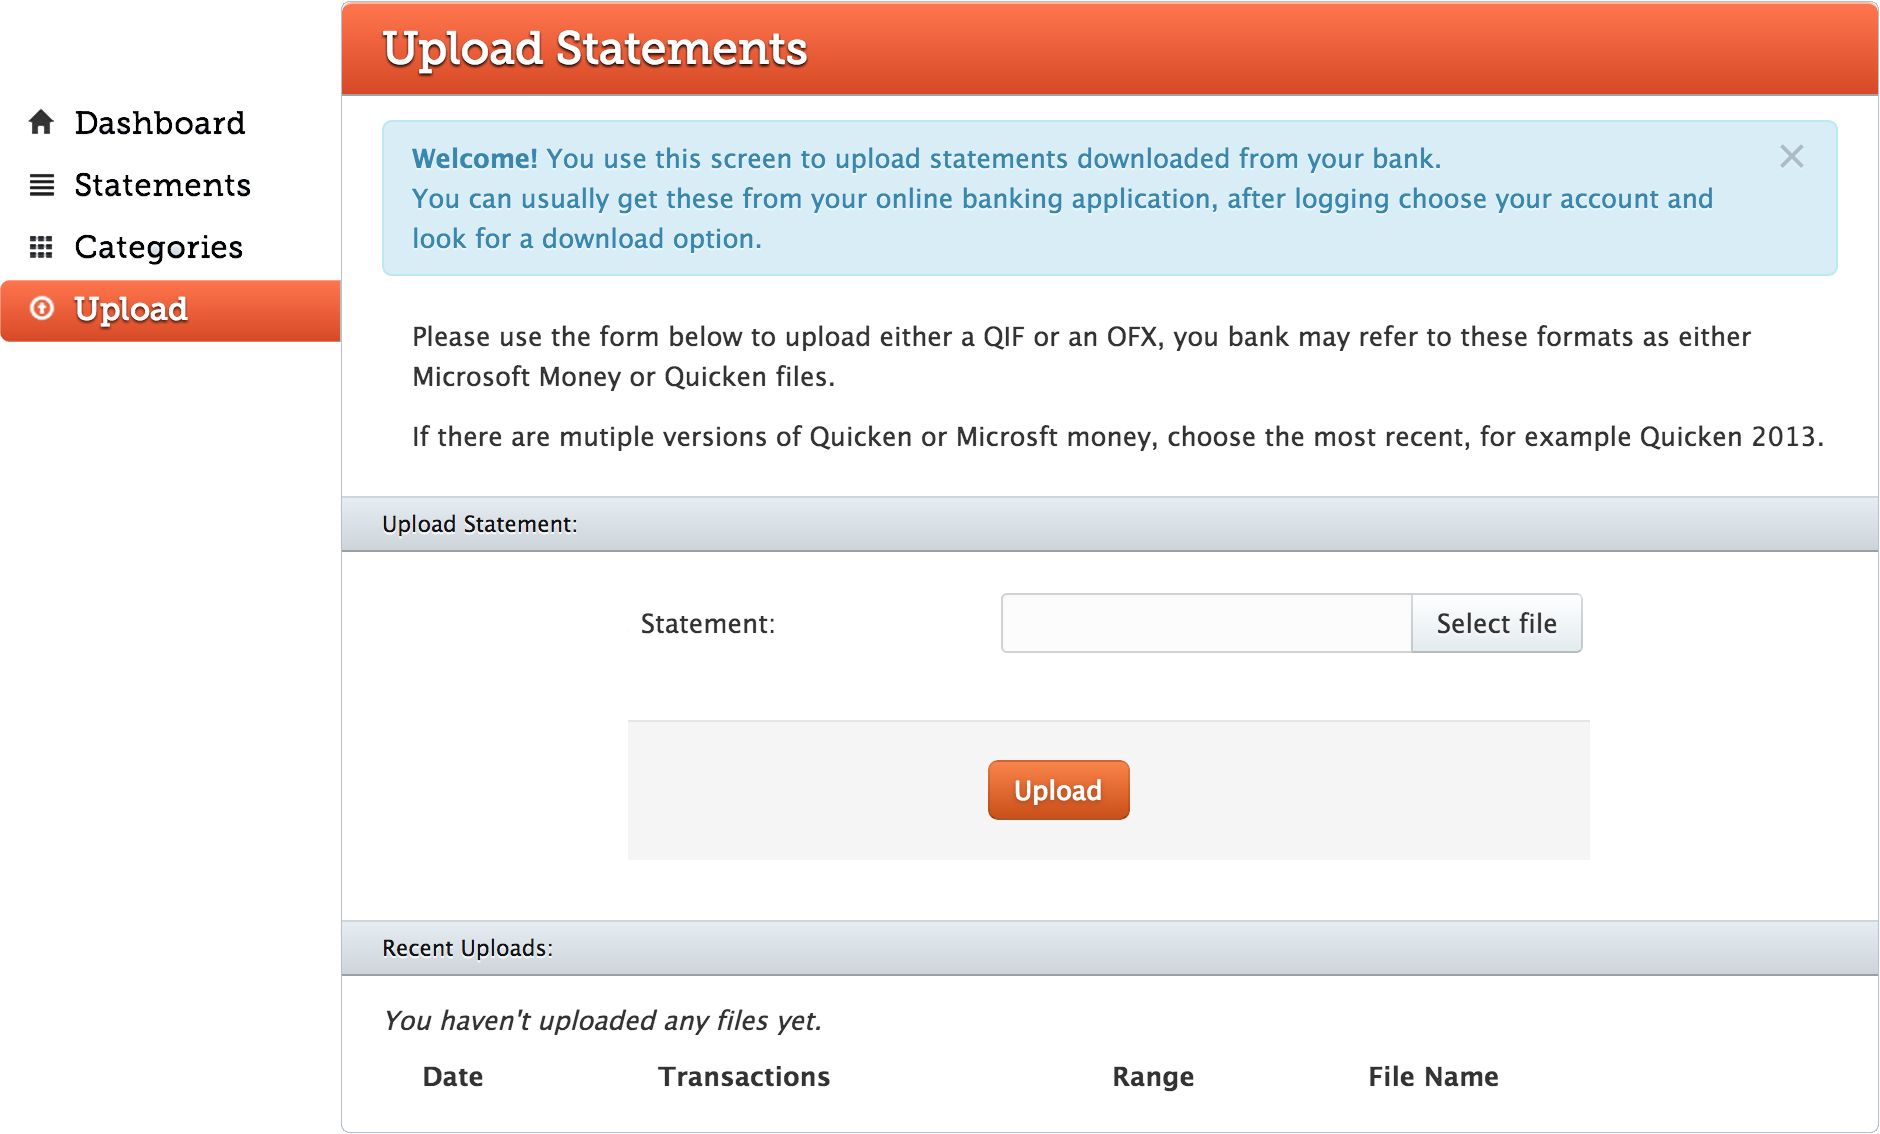
\includegraphics[width=0.8\textwidth]{screenshots/walkthrough/upload-empty}
\caption{The upload statement screen before any uploads}
\label{fig:uploadempty}
\end{figure}

Following the advice of the welcome page, the user opens the upload screen (Fig. \ref{fig:uploadempty}). As this is the first time user has opened this screen an information prompt is shown which explains the purpose of the page and reminds them that the files to upload can usually be found on their current banks Internet banking system.

\begin{figure}
\centering

\includegraphics[width=0.8\textwidth]{screenshots/walkthrough/upload-selected}
\caption{UI update following a file selection}
\label{fig:upload-selected}
\end{figure}

After downloading a statement from their, the user uploads the statement by clicks on the select file button and browsing their computer for the file. After confirming their selection the state of the file field changes (Fig. \ref{fig:upload-selected}) to allow checking of the uploaded file and to make it clear one is currently selected. Clicking the primary\footnote{Indicated in orange} upload button uploads the file to the server, which processes it, and refreshes the page.

\begin{figure}
\centering
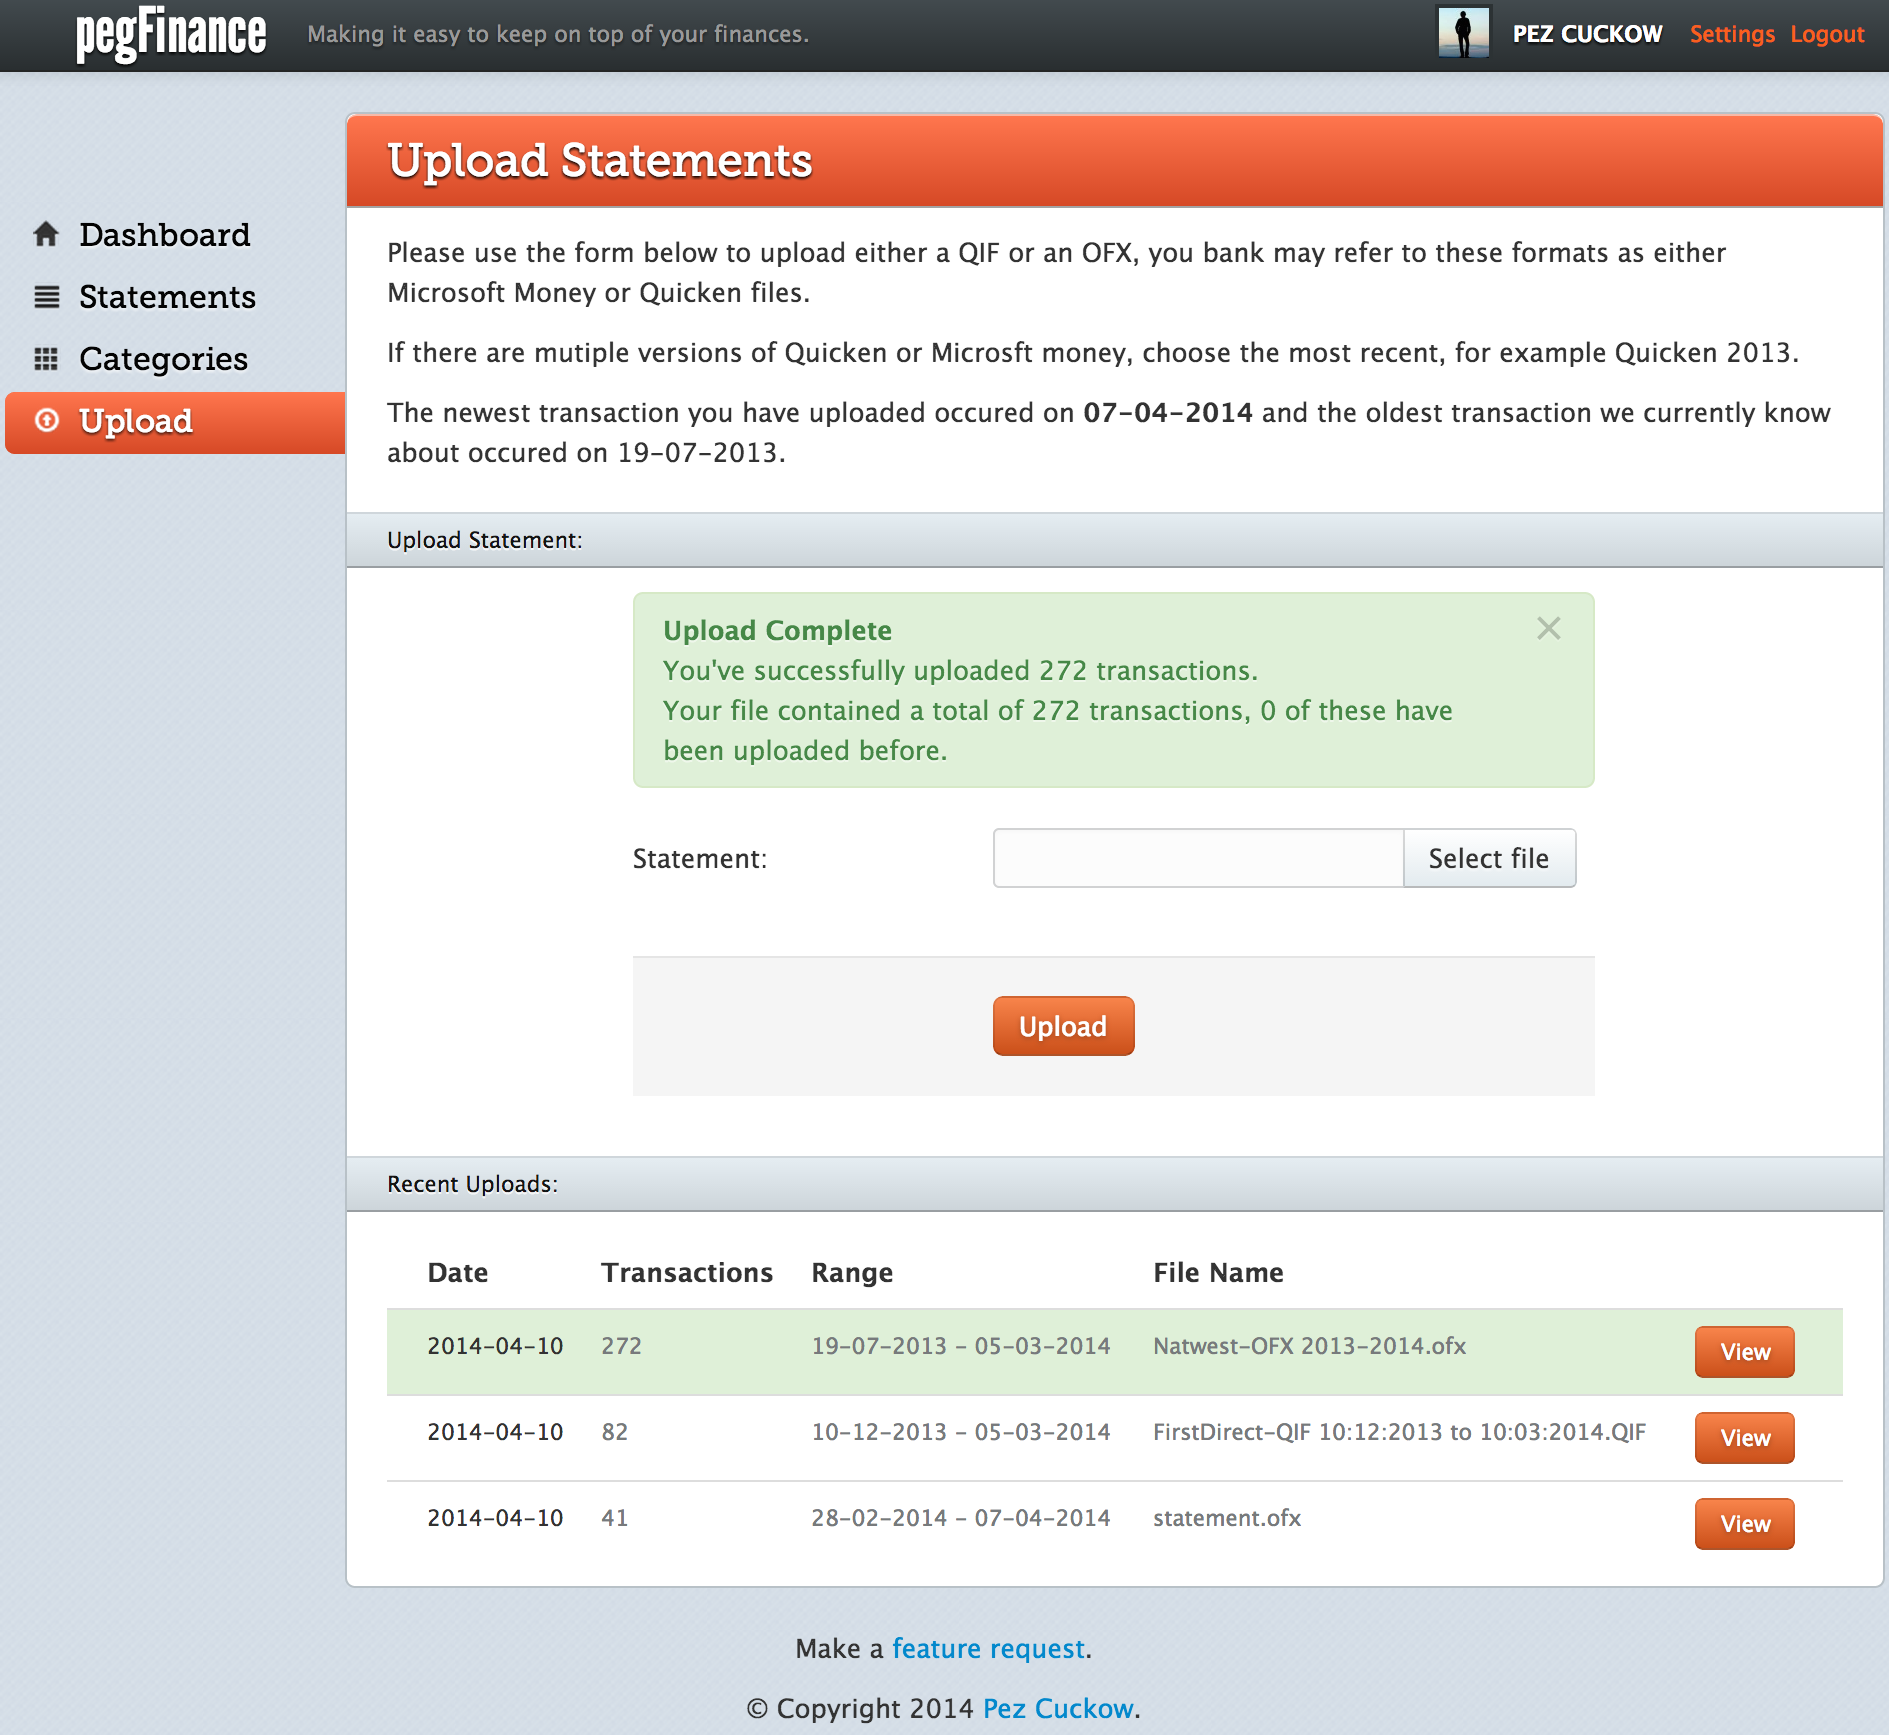
\includegraphics[width=0.8\textwidth]{screenshots/walkthrough/upload-complete}
\caption{The upload page, following successful file uploads}
\label{fig:upload-complete}
\end{figure}

On the new page (Fig. \ref{fig:upload-complete}), the state of the file upload is indicated above the form, containing a summary of the file uploaded and the uploaded file is highlighted in the recent uploads list, which includes an option to view the transactions uploaded as part of that statement. The highlight color, green, was used to indicate success. 

In addition a further piece of information has been added to the page introduction, the most recent transaction the system knows about is marked in bold, to save the user time when selecting a statement to download.

\begin{figure}
\centering

\includegraphics[width=0.8\textwidth]{screenshots/walkthrough/upload-already}
\caption{Upload confirmation following a duplicate file}
\label{fig:upload-duplicate}
\end{figure}

If the user uploads a file containing no new transactions (all previously uploaded), the confirmation prompt indicates this and it uses the colour yellow to indicate a warning (Fig. \ref{fig:upload-duplicate}).

\begin{figure}
\centering
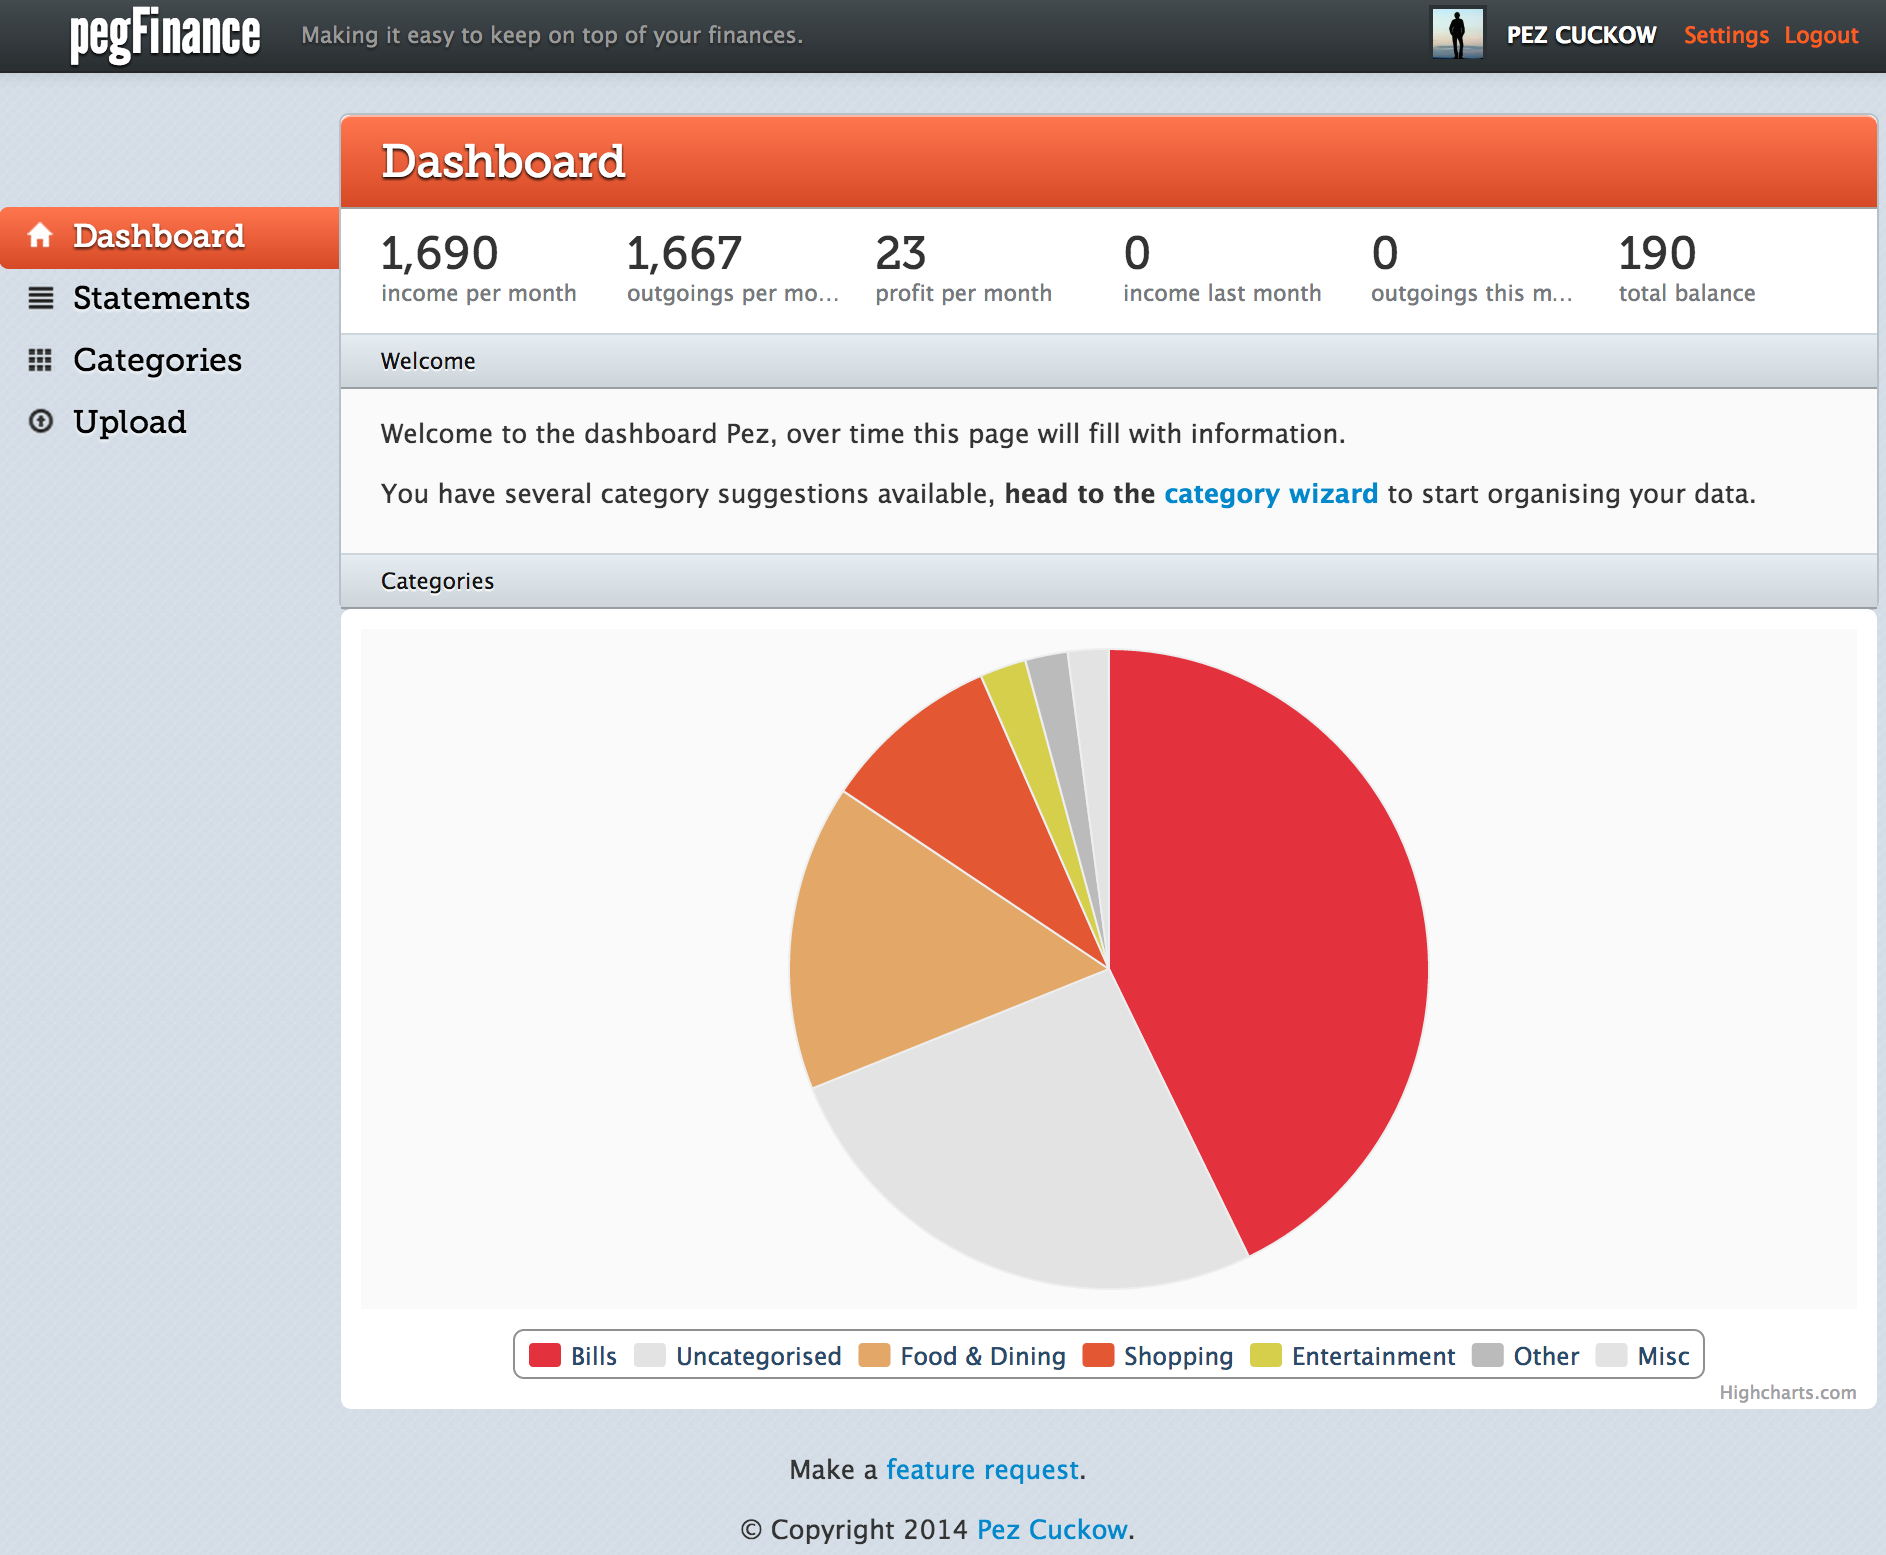
\includegraphics[width=0.8\textwidth]{screenshots/walkthrough/dashboard-full}
\caption{Welcome screen following statement uploads}
\label{fig:welcome-full}
\end{figure}

\begin{figure}
\centering
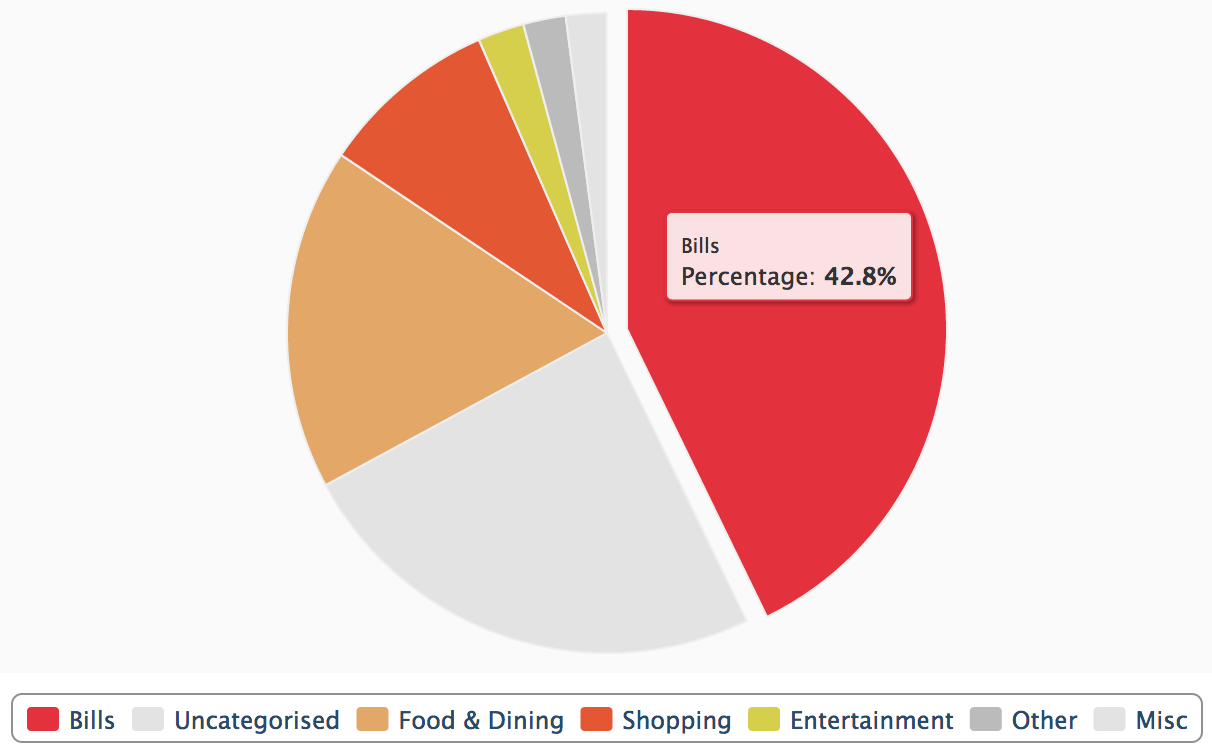
\includegraphics[width=0.8\textwidth]{screenshots/walkthrough/piecharthover}
\caption{Additional pie chart detail}
\label{fig:piecharthover}
\end{figure}

On returning to the welcome screen, the dashboard is now full of information\footnote{Fictional information used throughout out this walkthrough} (Fig. \ref{fig:welcome-full}). It provides an overview of the average income and outgoings per month, along with an indication of the users `profit' since the first transaction the application knows about. 

Most notably, the dashboard also includes an interactive pie chart, which gives an indication as to which categories most of their money is spent. On hover the chart gives the actual percentage of the overall expenditure \ref{fig:piecharthover}, and on click opens a page which lists all the transactions in that category.

If the system has suggestions for uncategorised transactors, a notification suggesting they visit the category (or suggestion) wizard is shown.

\section{Suggestion Wizard}
\label{subsection:suggestion-wizard-walkthrough}.

\begin{figure}
\centering
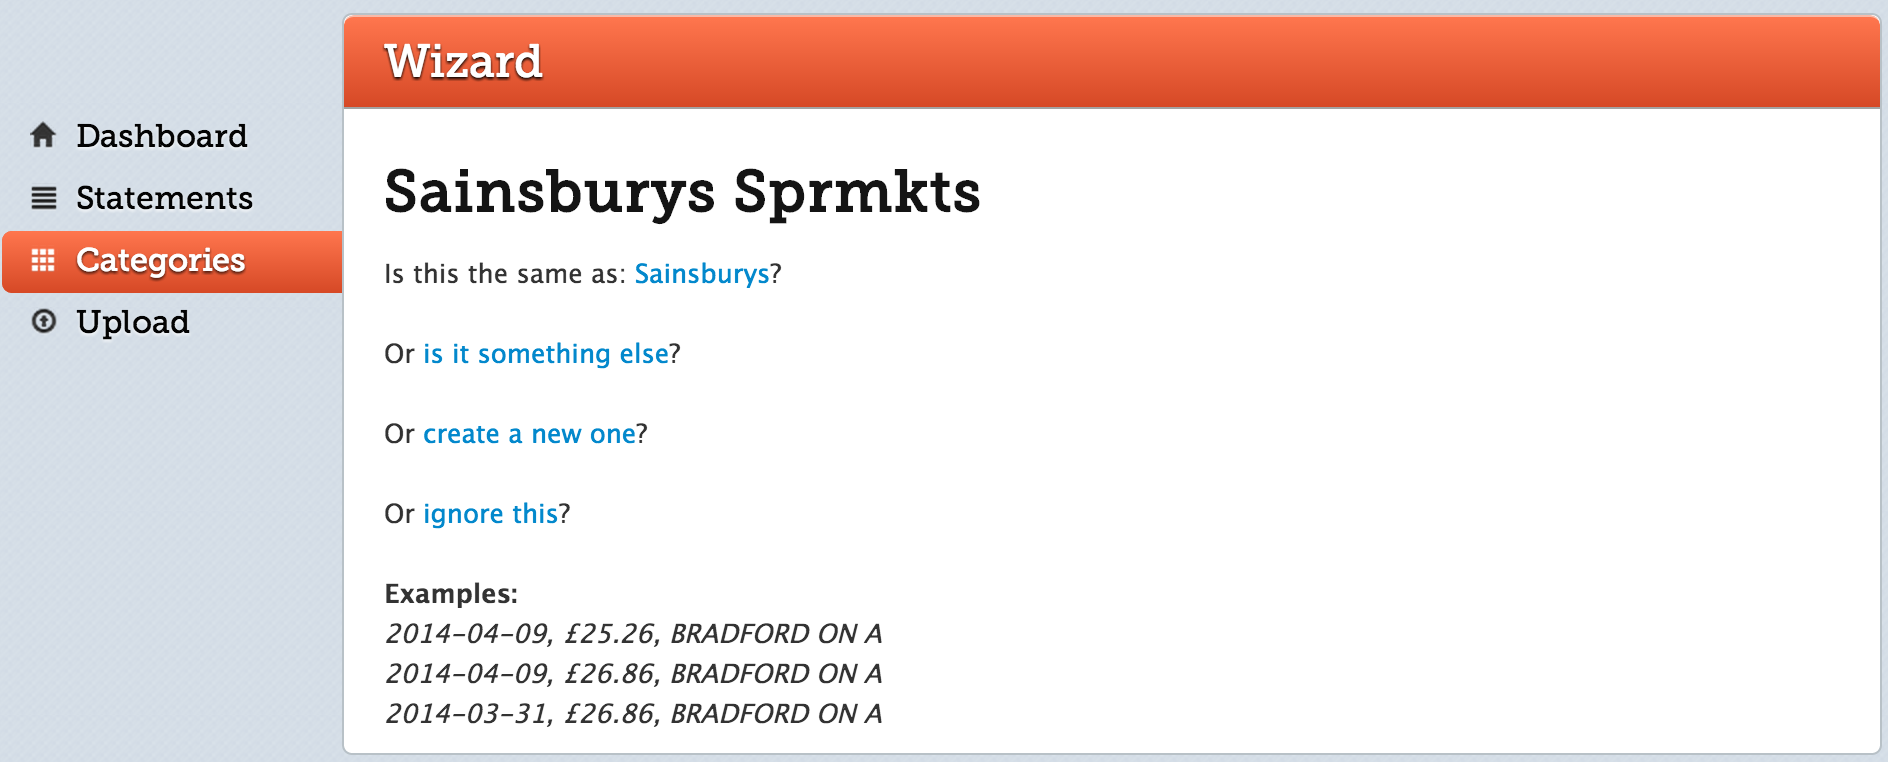
\includegraphics[width=0.8\textwidth]{screenshots/walkthrough/wizard-screen}
\caption{Suggestion wizard main screen, showing suggestions for a reference to Sainsbury's}
\label{fig:wizard-screen}
\end{figure}

The suggestion wizard steps the user though all unmapped and uncategorised references (Fig \ref{fig:wizard-screen}. It starts with the transactor they frequent the most often and prompts them to provide the mapping, either by following a suggestion, creating a new transactor or manually searching for a match.

\begin{figure}
\centering
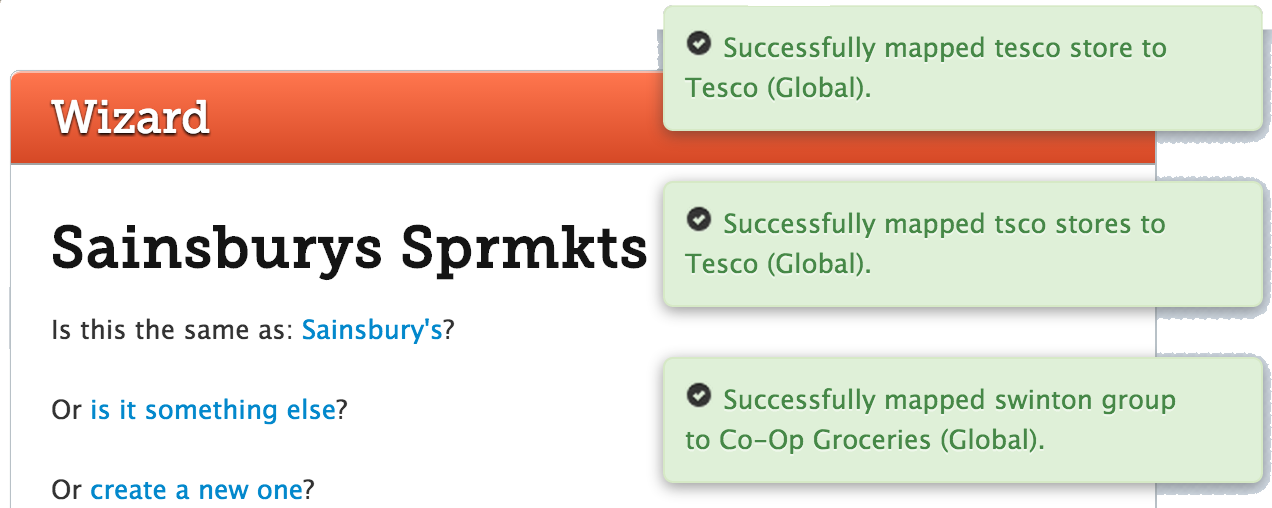
\includegraphics[width=0.8\textwidth]{implementation/suggestion-notification}
\caption{Notifications shown after completing a sucessfully}
\label{fig:suggestion-complete-notification}
\end{figure}

Completing the mapping, forwards the user to the next unmapped reference, providing confirmation the new mapping has been created as a notification which disappears after a few seconds \ref{suggestion-complete-notification}, and the process repeats.

\begin{figure}
\centering
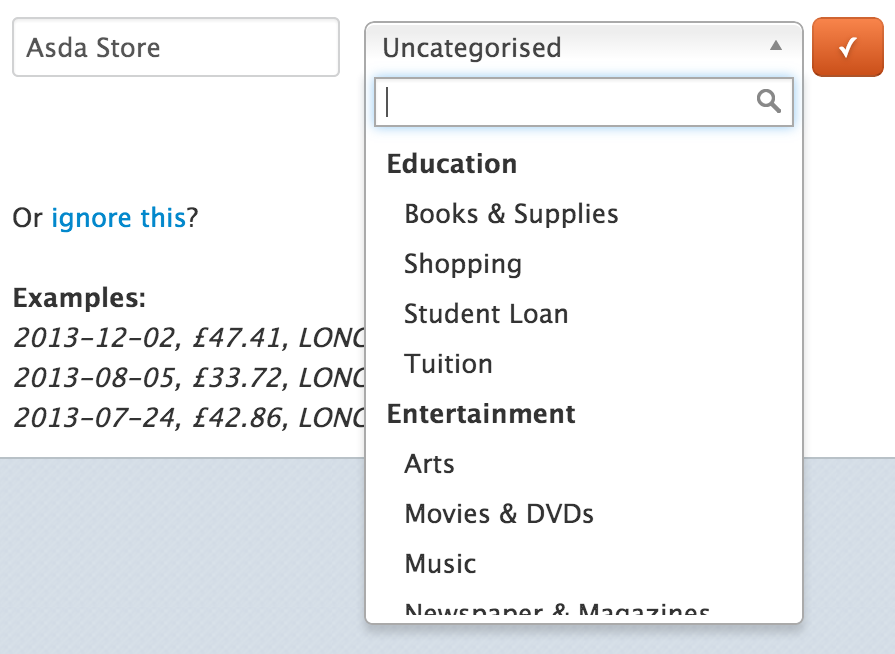
\includegraphics[width=0.8\textwidth]{screenshots/walkthrough/wizard-create-dropdown}
\caption{Creating a new Transactor and selecting a category}
\label{fig:create-new-transactor}
\end{figure}

\begin{figure}
\centering
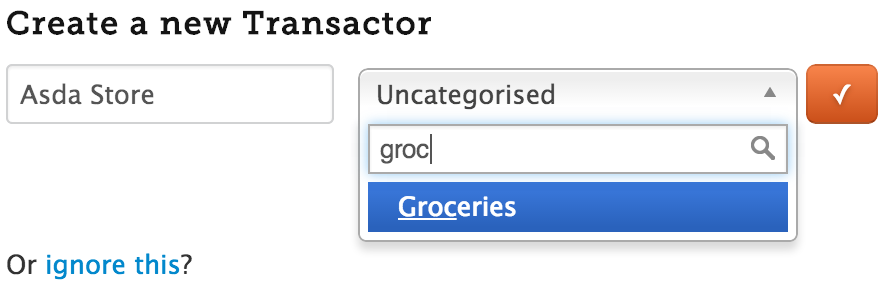
\includegraphics[width=0.8\textwidth]{screenshots/walkthrough/wizard-create}
\caption{Selecting a category using the autocomplete feature}
\label{fig:dropdown-autocomplete}
\end{figure}

\begin{figure}
\centering
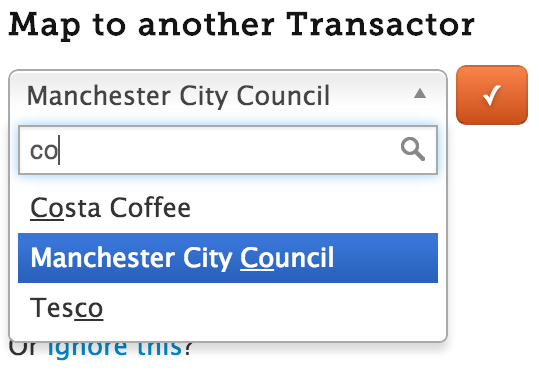
\includegraphics[width=0.8\textwidth]{screenshots/walkthrough/wizard-map}
\caption{Searching for an existing Transactor using autocomplete}
\label{fig:wizard-map-dropdown}
\end{figure}

The suggestions wizard went through several iterations of user interface enhancements, designed to make it easier to use.
%
For example, when creating a new transactor (Fig. \ref{fig:create-new-transactor}) the system automatically fills in the name field with a pre-formatted version of the reference and the category selection is performed through an upgraded dropdown menu. The dropdown has been upgraded from the standard dropdown found on many websites using client side javascript and provides auto-completion, fuzzy matching, as well as the ability to select a category grouping instead of an exactly category, for example entertainment over Movies \& DVD's (Fig. \ref{fig:dropdown-autocomplete}. A similar dropdown is also used when searching for an existing transactor (Fig. \ref{fig:wizard-map-dropdown}.

After completing the wizard by mapping or ignoring all the unmapped references, the user is congratulated and a hint is given that they should head to the transaction summary page, which includes their monthly expenditure predictions.

\section{Transaction Overview}

\begin{figure}
\centering
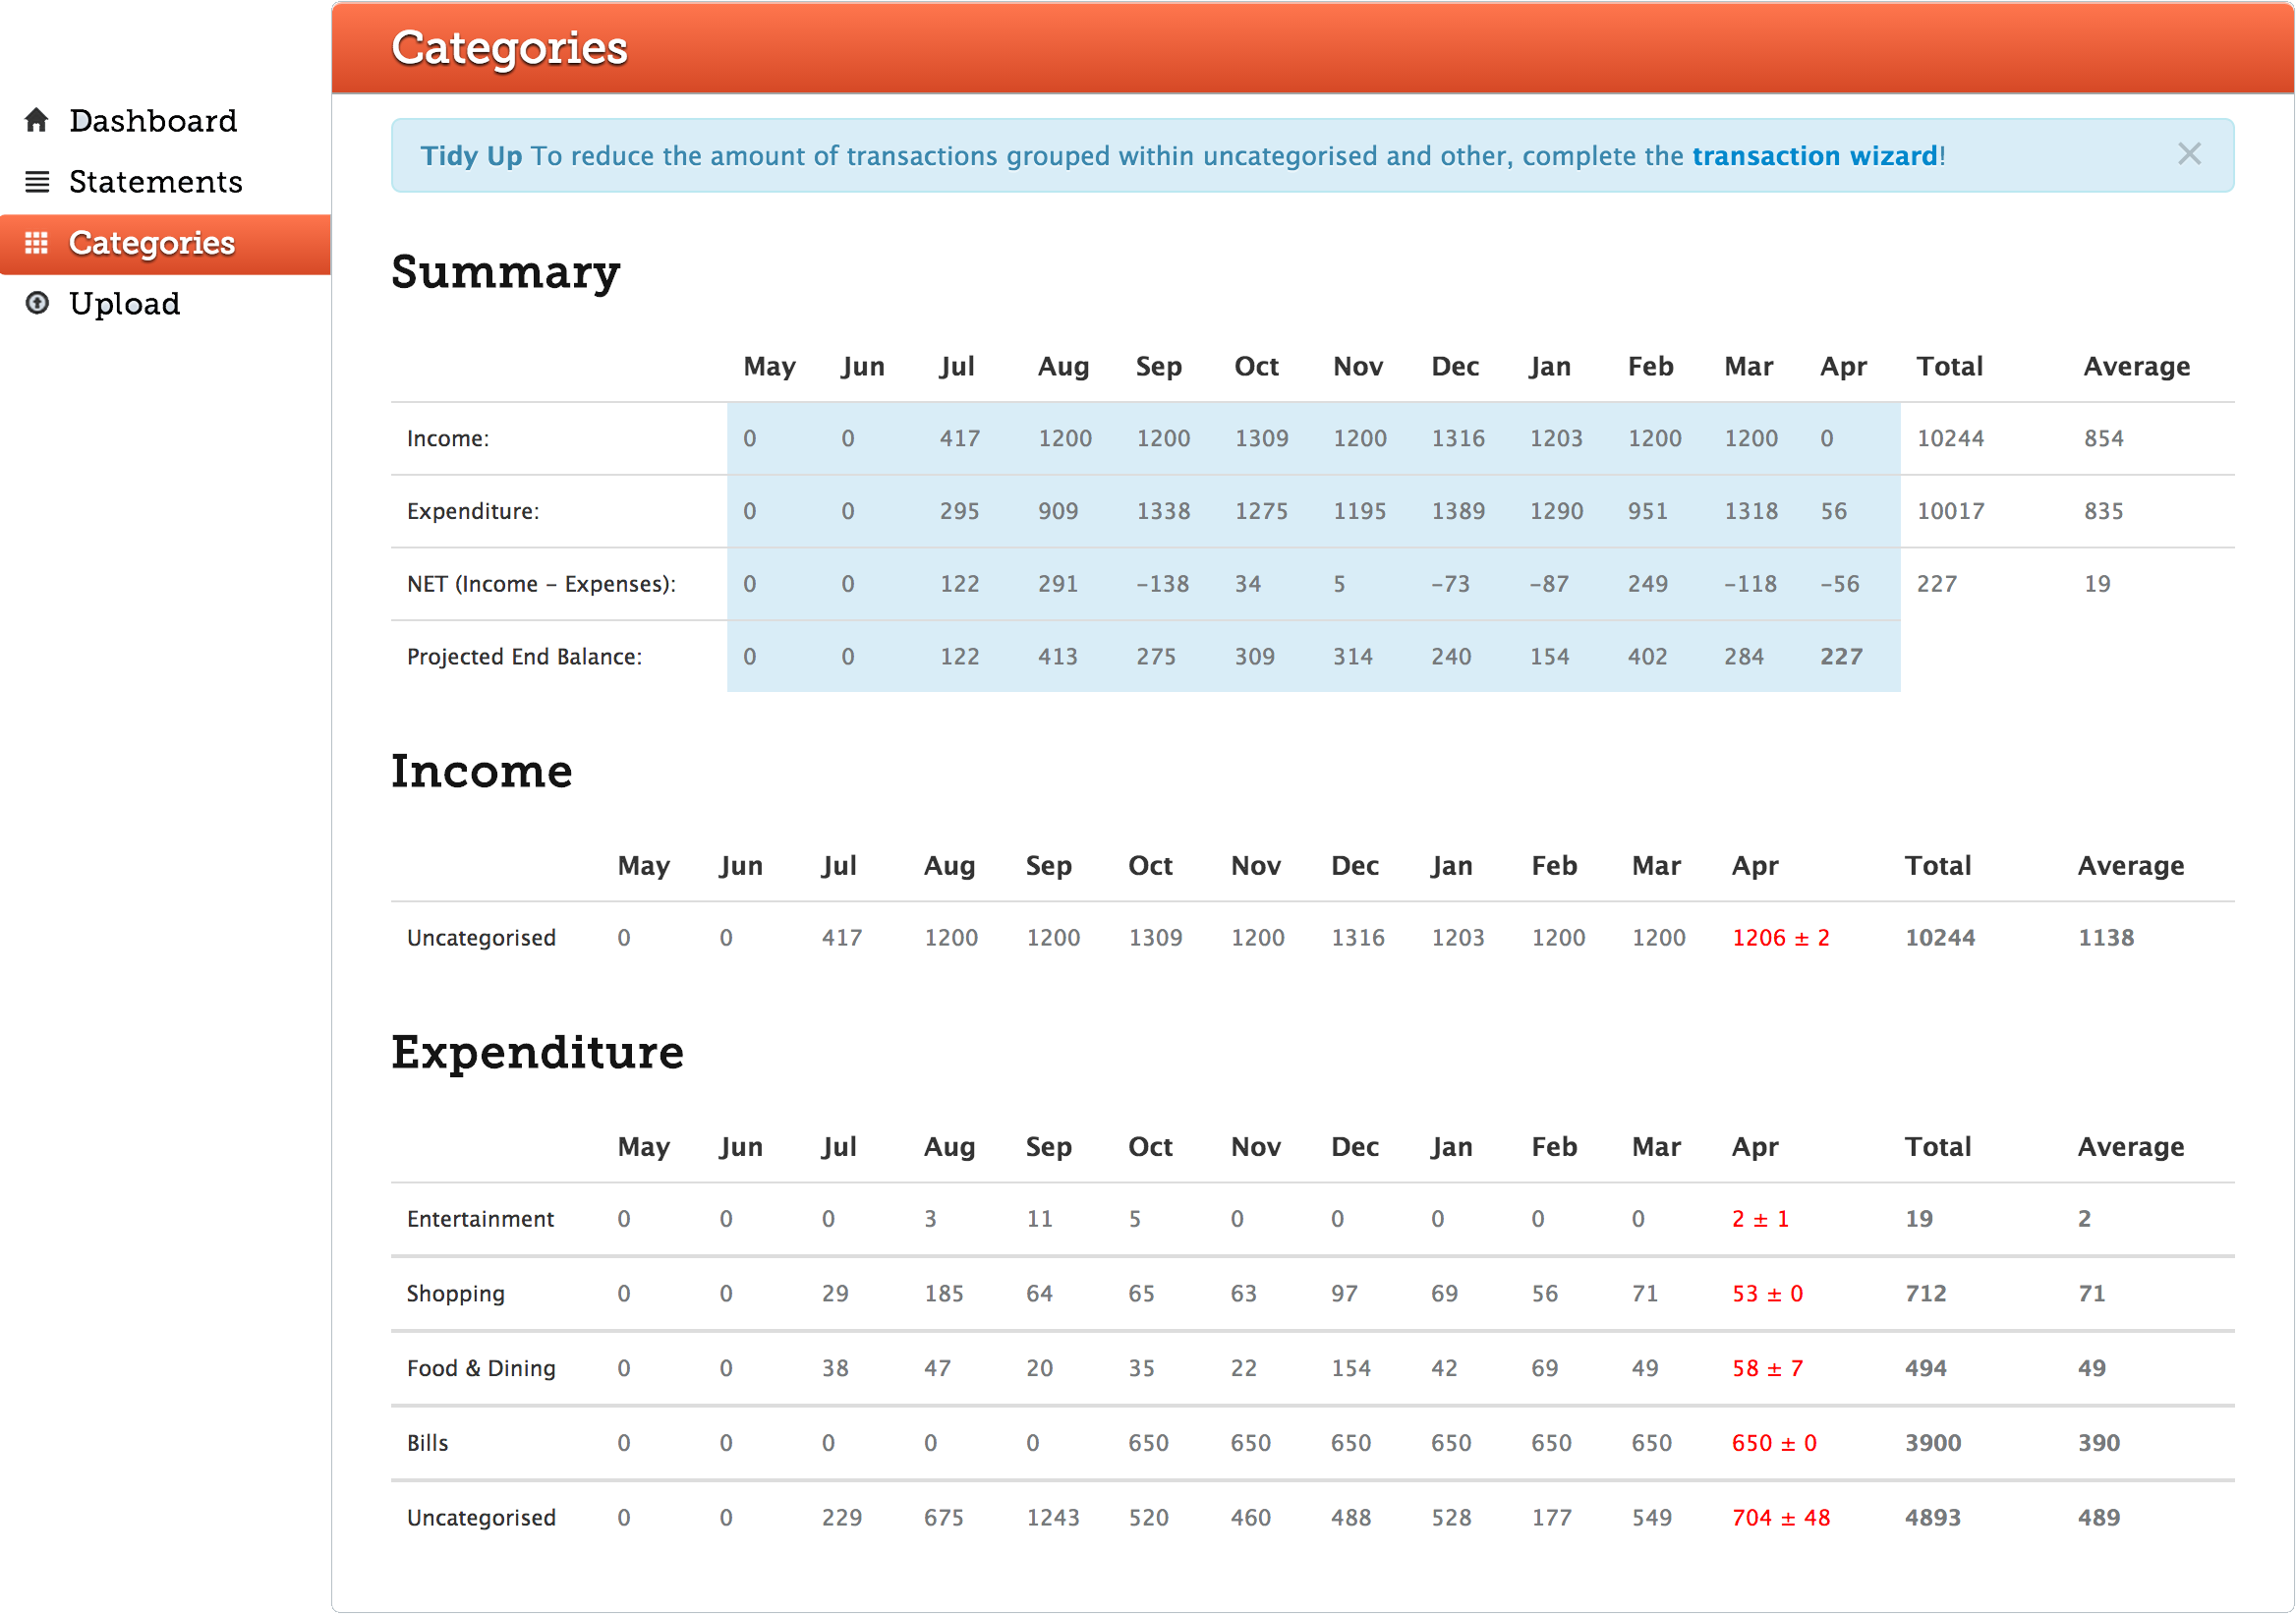
\includegraphics[width=0.8\textwidth]{screenshots/walkthrough/transaction-overview}
\caption{The transaction overview screen, which shows expenditure per month and a prediction (in red) for next month}
\label{fig:transaction-overview}
\end{figure}

The transaction overview screen shows spending per month in each of the categories and a the prediction for next month made using the machine learning techniques outlined in \autoref{section:prediction-system} (Fig. \ref{fig:transaction-overview}). At the top of the screen a summary of the total income, expenditure and net profit for each month is shown. The rest of the page is split into two sections, representing money coming into and leaving the users account. In the example shown the user hasn't mapped all of their references and so some transactions are listed under uncategorised, a hint is placed at the top of the screen reminder users to visit the category wizard. 

\begin{figure}
\centering
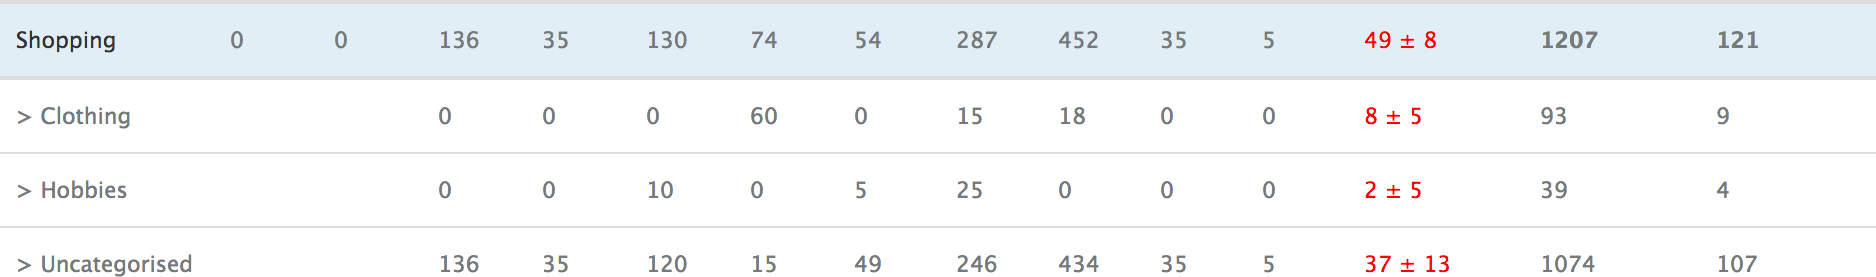
\includegraphics[width=0.8\textwidth]{screenshots/walkthrough/transaction-subcategories}
\caption{The subcategories being used to make up a category in the overview}
\label{fig:transaction-subcategories}
\end{figure}
.png

Clicking on any of the rows in the table reveals the subcategories and their associated values that are being used to produce the row, using an animated `slide-down' effect \ref{fig:transaction-subcategories}. 

\section{Viewing Statements}
\begin{figure}
\centering
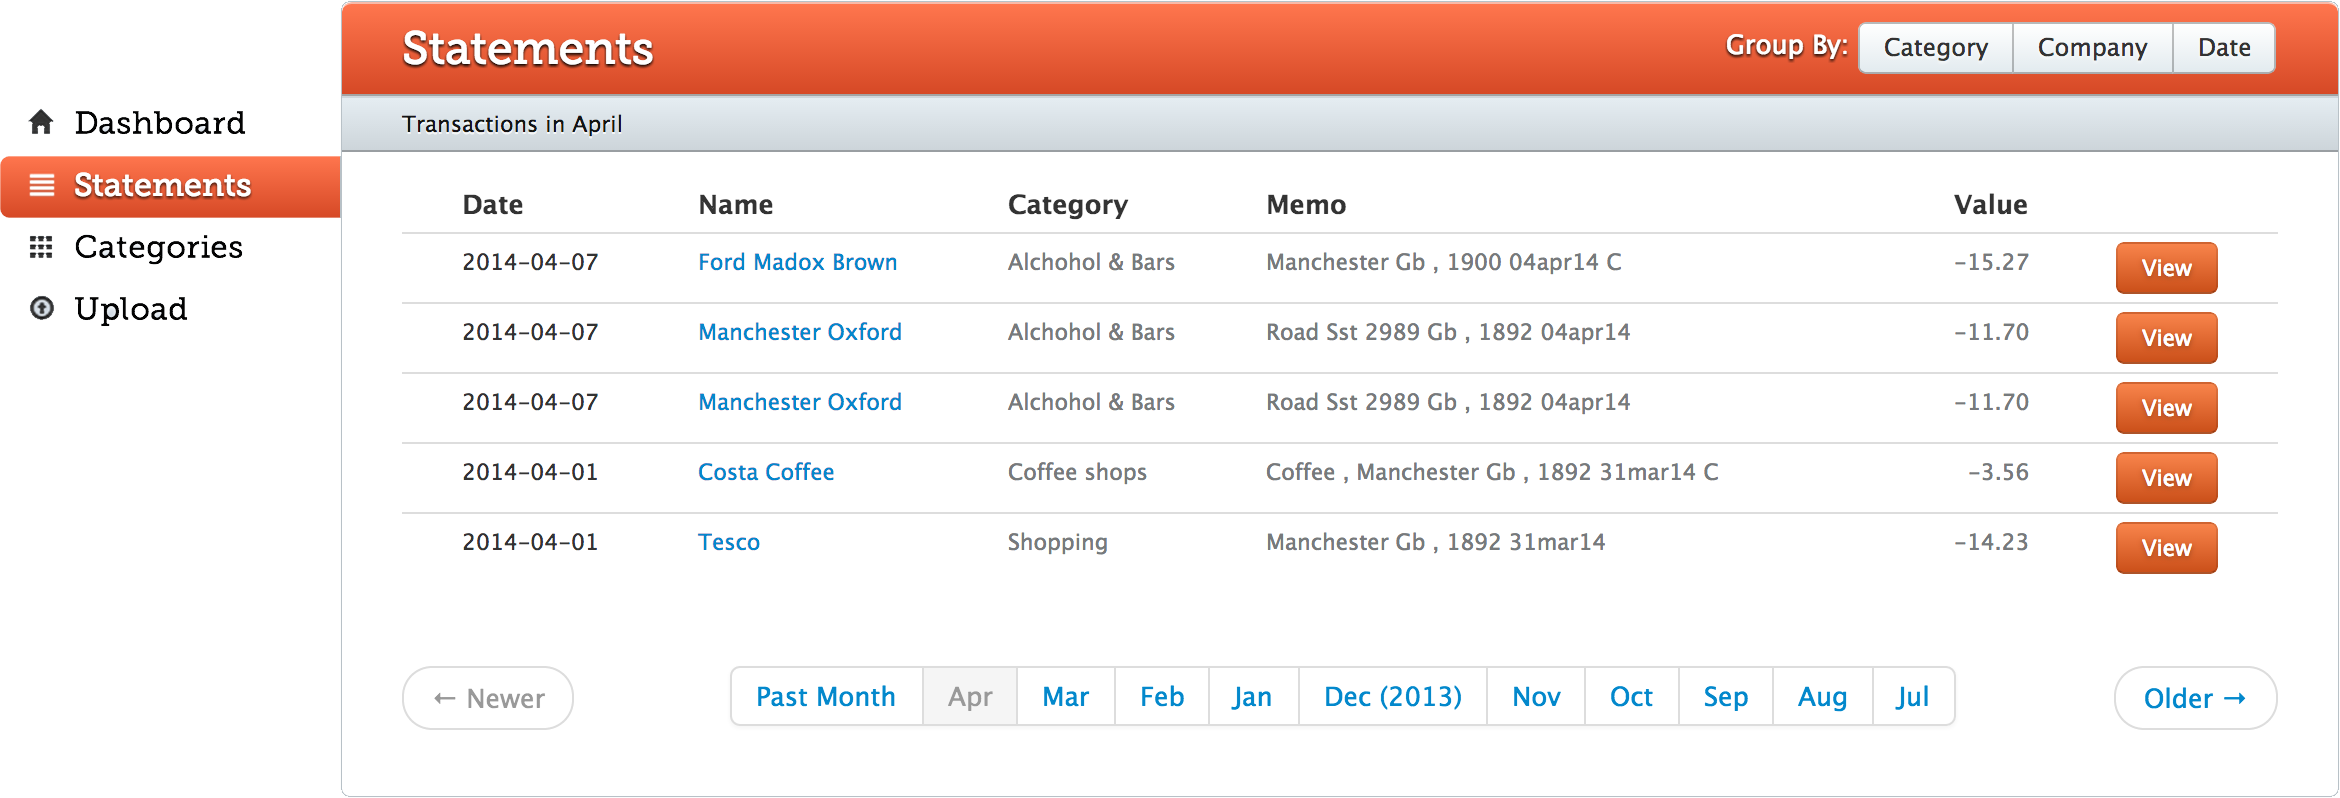
\includegraphics[width=0.8\textwidth]{screenshots/walkthrough/statement-view}
\caption{The statement view}
\label{fig:statement-view}
\end{figure}

\begin{figure}
\centering
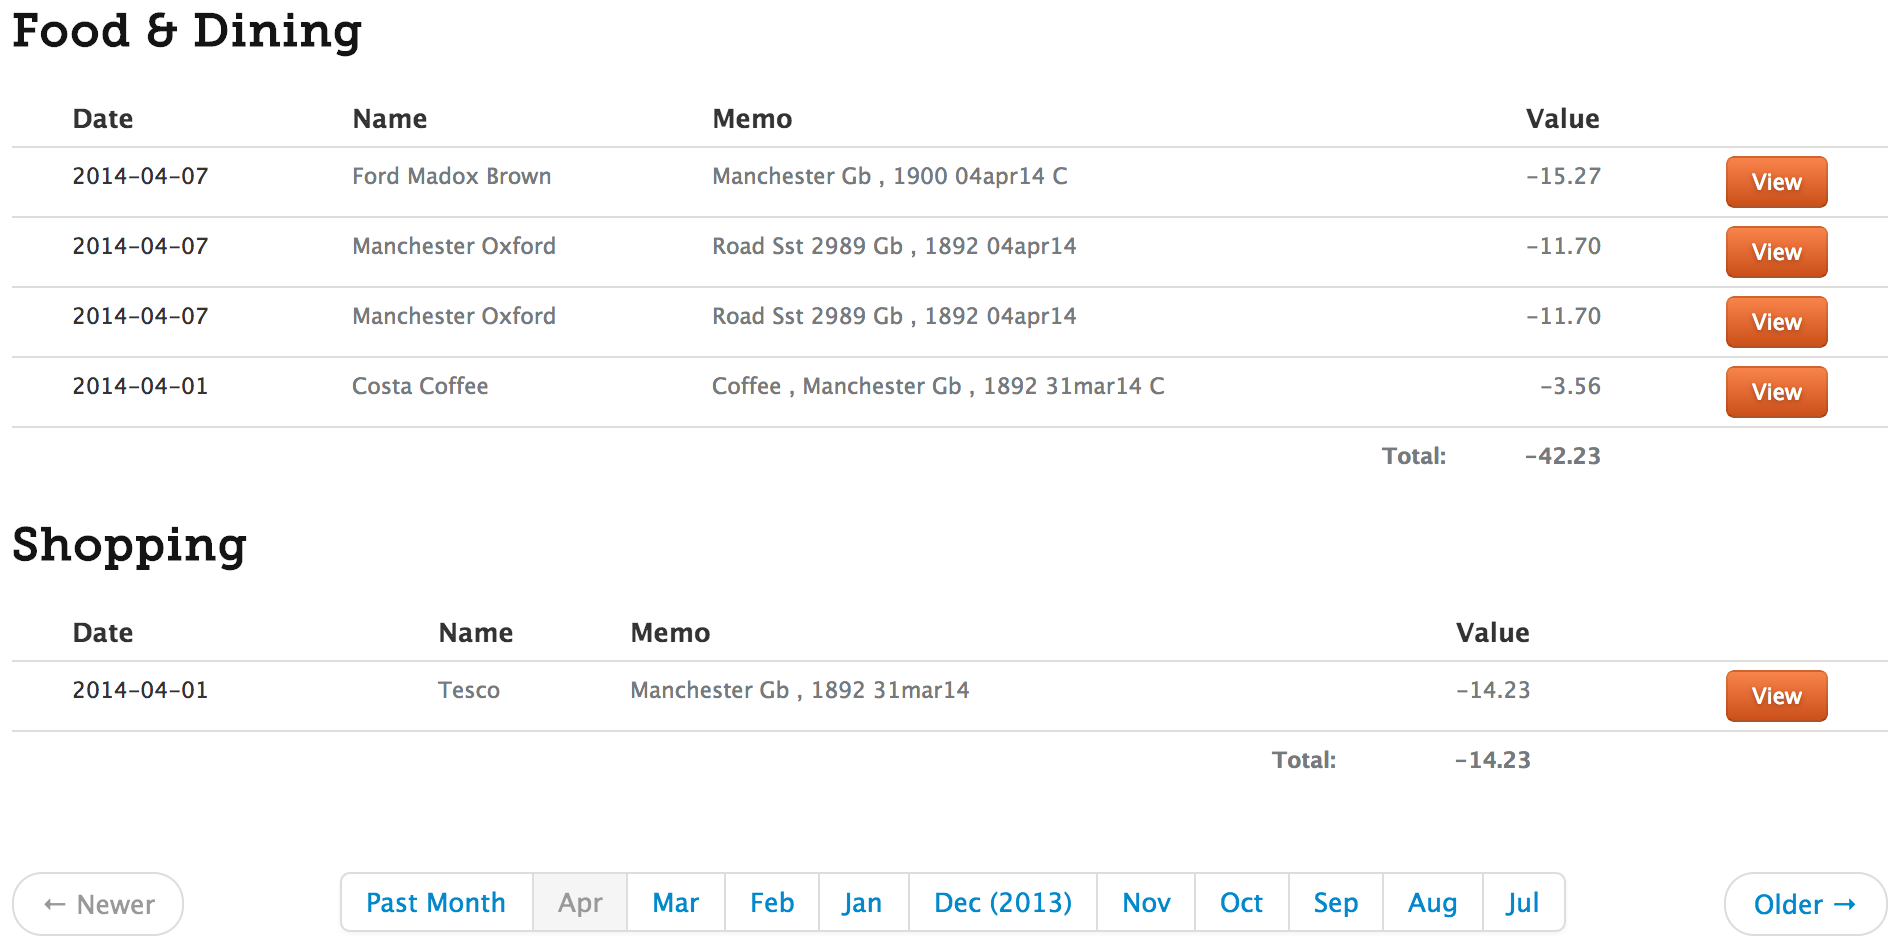
\includegraphics[width=0.8\textwidth]{screenshots/walkthrough/statements-group-category}
\caption{Grouping the statement by category}
\label{fig:statements-group-category}
\end{figure}

\begin{figure}
\centering
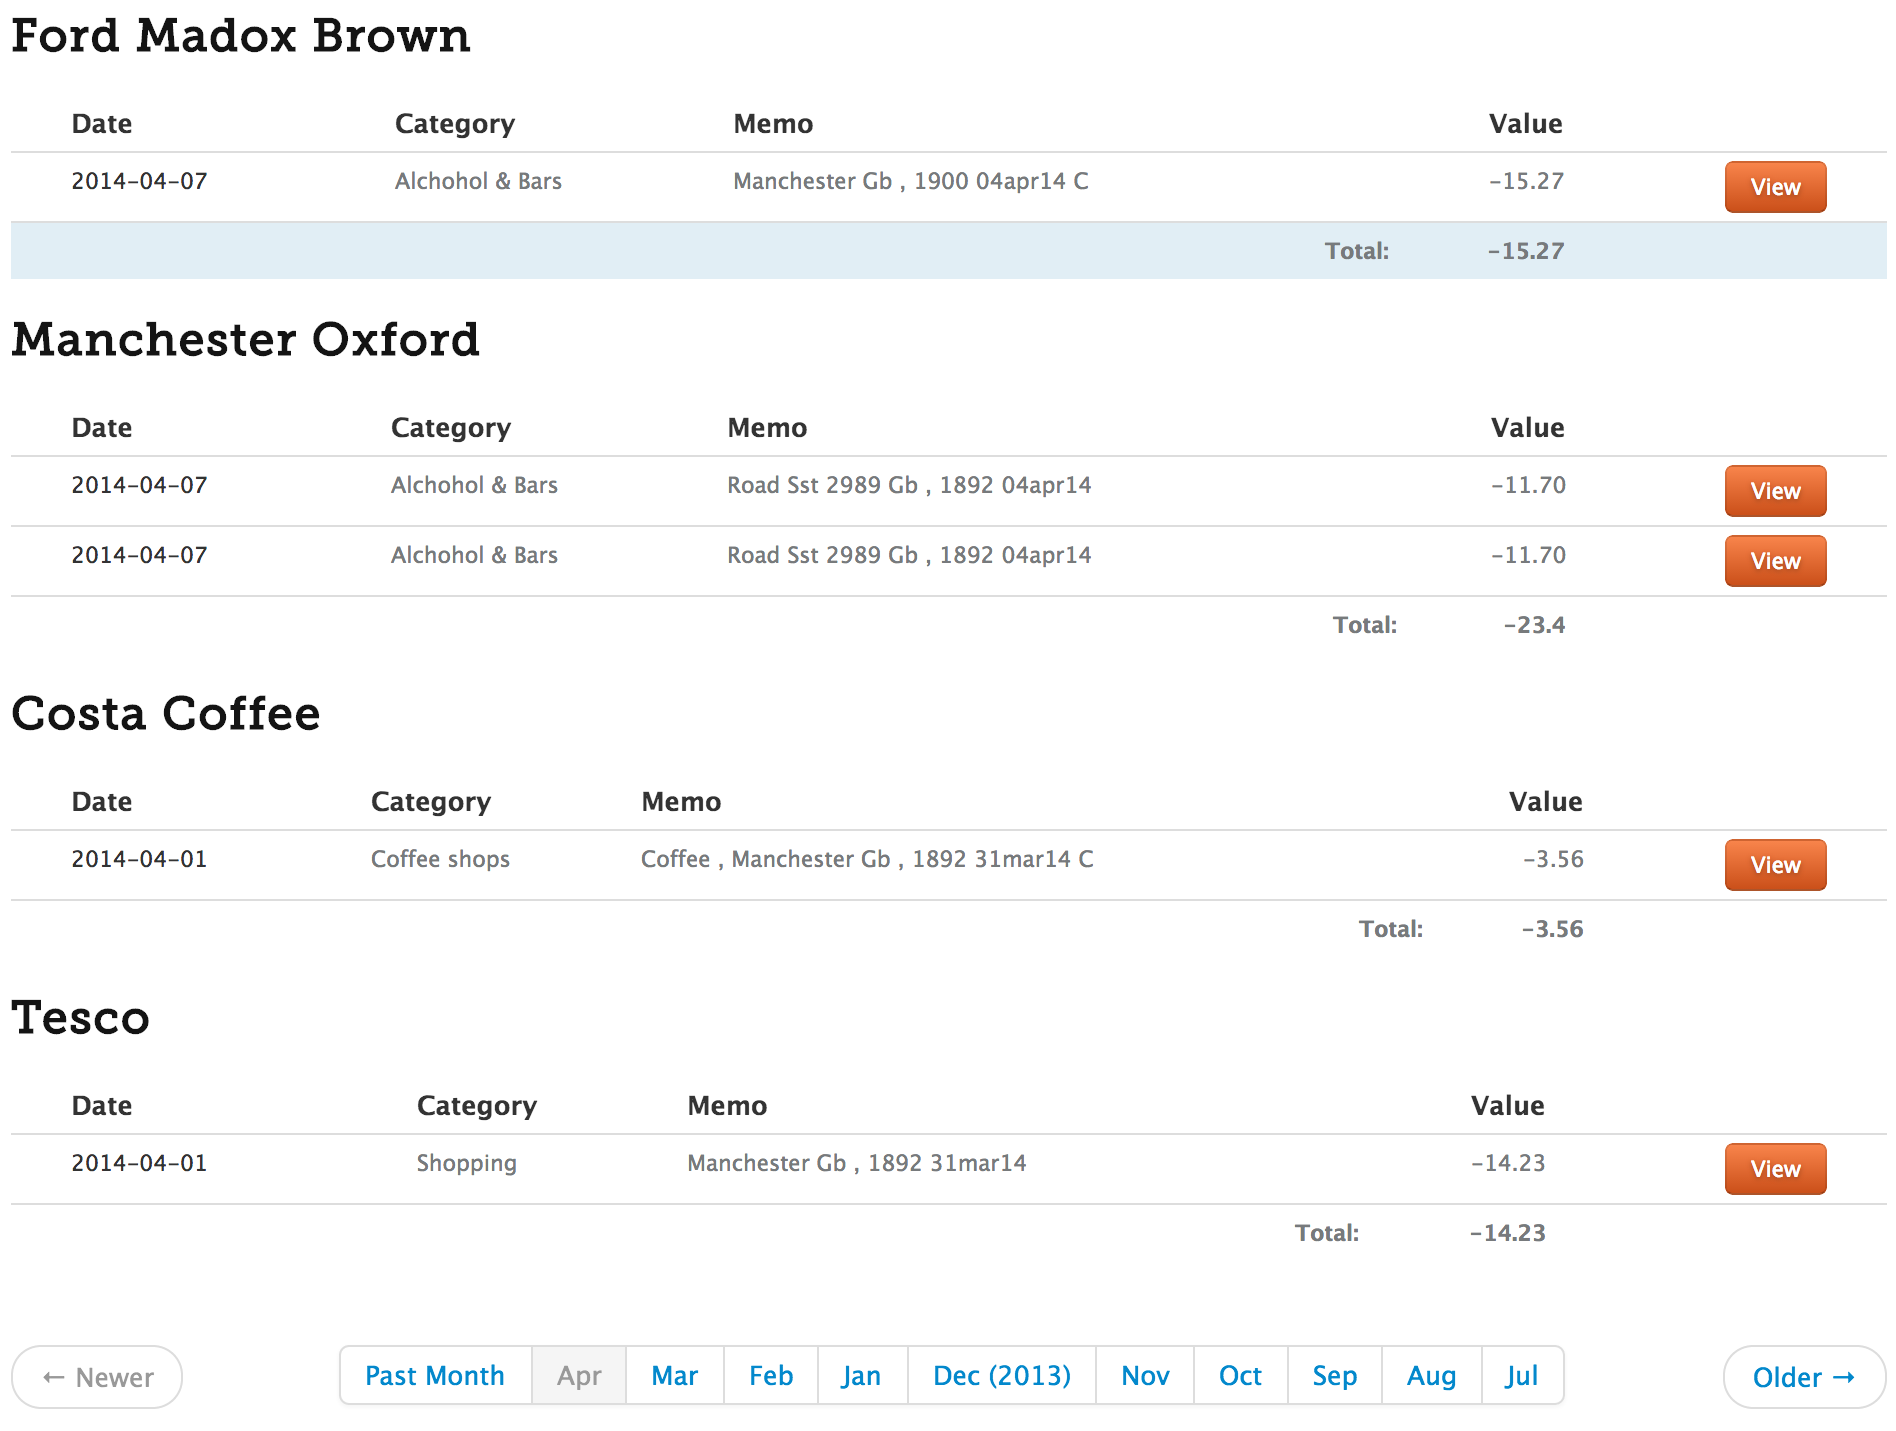
\includegraphics[width=0.8\textwidth]{screenshots/walkthrough/statements-groupby-company}
\caption{Grouping the statement by category}
\label{fig:statements-groupby-company}
\end{figure}

The application also provides an easy way to view historical spending organised by month (Fig \ref{fig:statement-view}). The transactions in each month can be grouped by category, transactor or date to give a more detailed idea of how money is being spent (Figs. \ref{fig:statements-group-category} and \ref{fig:statements-groupby-company}).

\begin{figure}
\centering
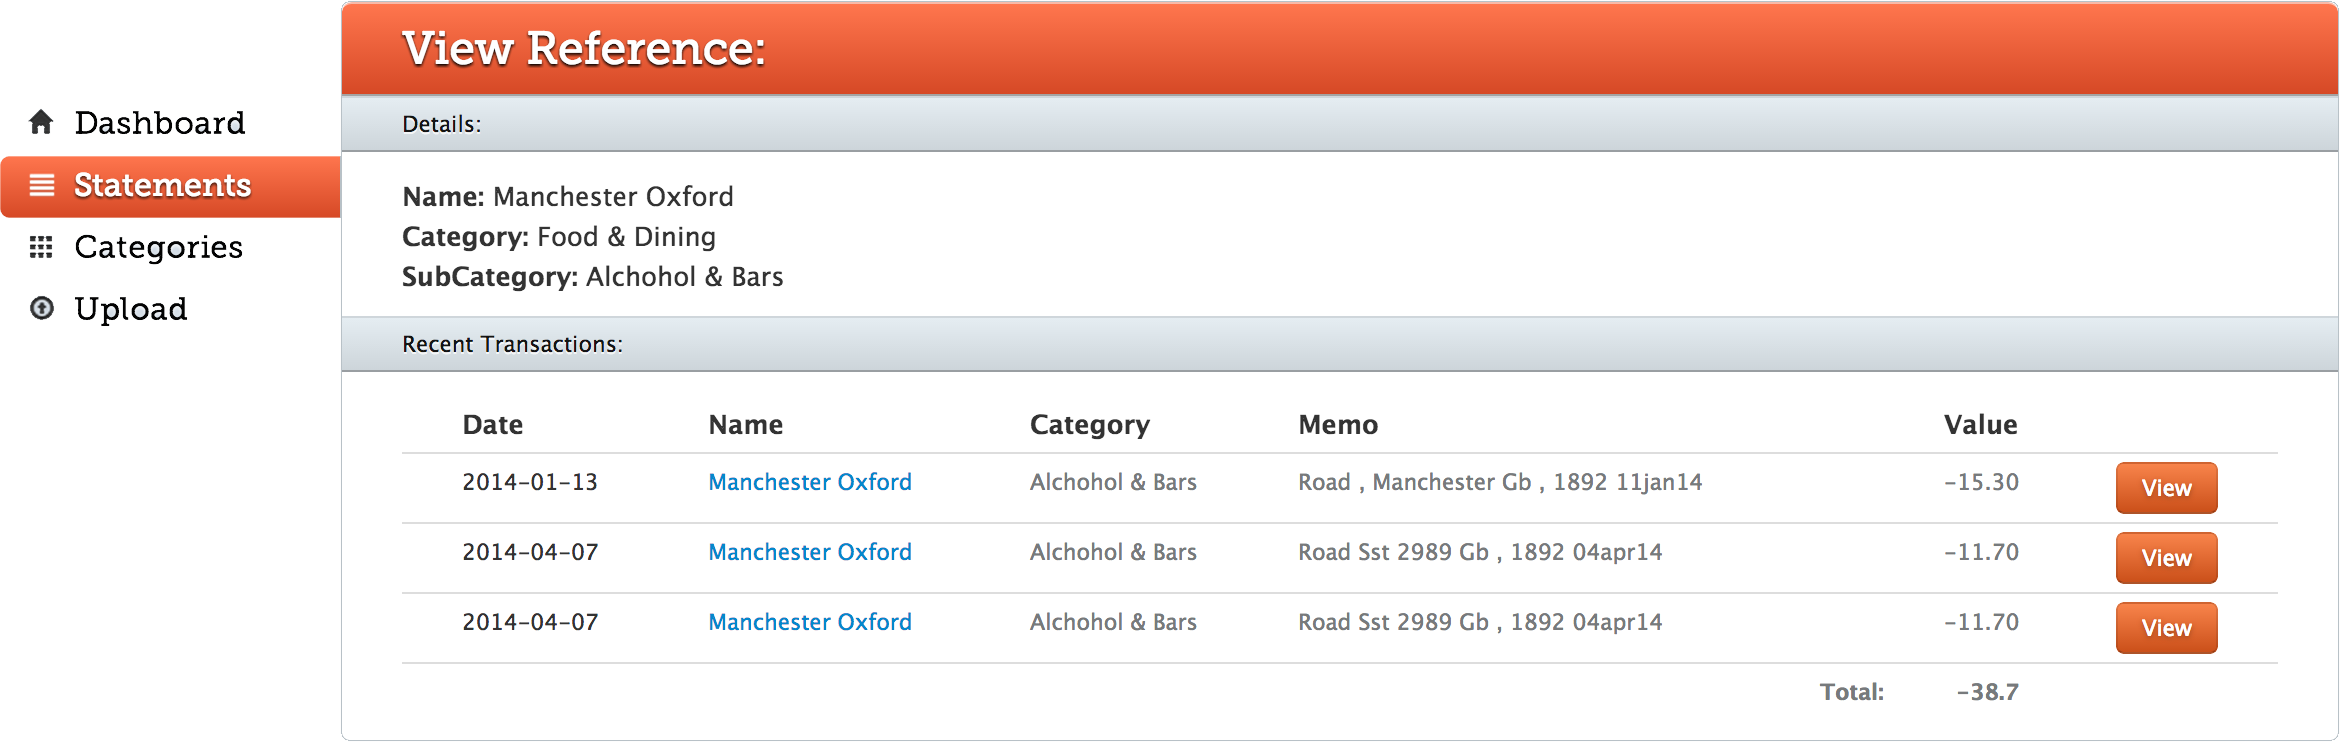
\includegraphics[width=0.8\textwidth]{screenshots/walkthrough/view-reference}
\caption{Recent transactions at a particular transactor}
\label{fig:view-reference}
\end{figure}

\begin{figure}
\centering
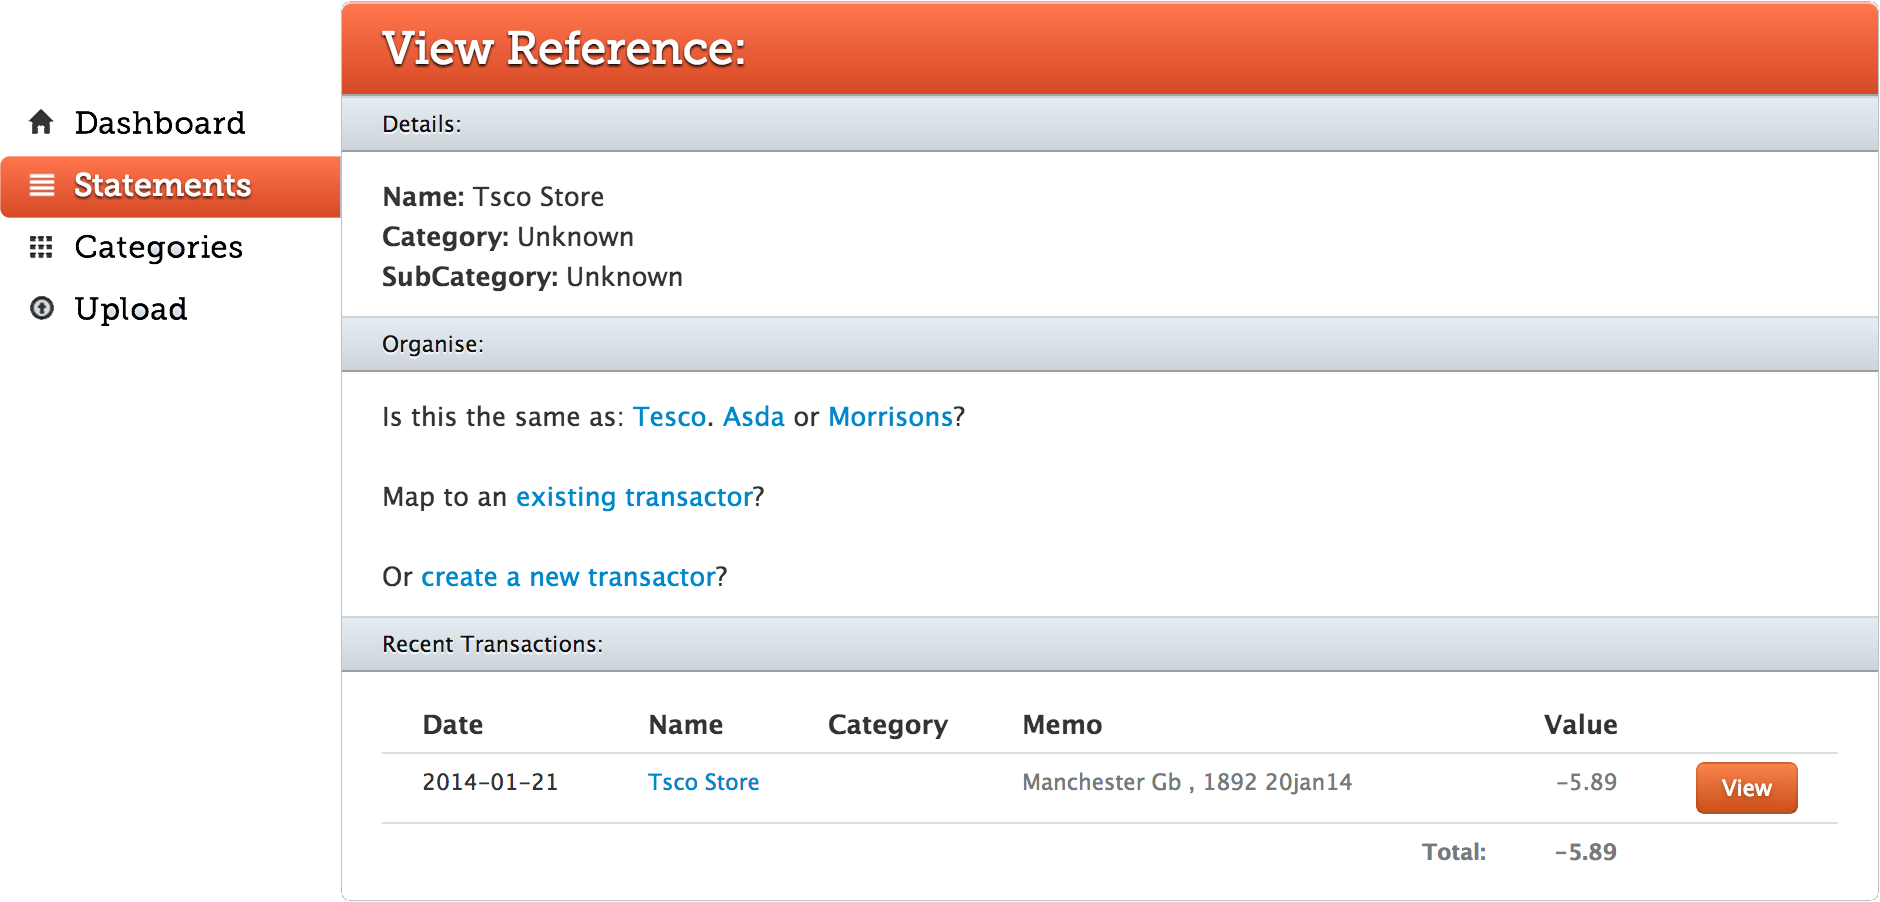
\includegraphics[width=0.8\textwidth]{screenshots/walkthrough/view-reference-unmapped}
\caption{Viewing an unmapped reference}
\label{fig:view-reference-unmapped}
\end{figure}

A user can also view particular transactor or reference, which includes the references category and a summary of recent transactions (Fig. \ref{fig:view-reference}). If the reference is not yet mapped, options similar to those shown in the suggestions wizard are listed enabling them to map the reference correctly (Fig. \ref{fig:view-reference-unmapped}). 

\section[Responsive Design]{Responsive Web Design}
A key feature of the application is being able to access it at any time from any device, particularly when taking into account the rapid increase in the use of mobile devices.  Interacting with a website on a smartphone or tablet is not the same as interacting using a computer, due to the smaller screen size and use of touch over a mouse.

Forbes reported that 24\% of their 2013 website visits came from mobiles and 13\% from tablets, down from a total of 15\% in 2012. particularly with the high percentage of website visits coming from mobile devices \parencite{steimle2013responsive}.

In order to ensure the project is accessible from a variety of different devices the core UI uses Responsive Web Design (RWD) to layout the website differently depending on the screen size of the device to ensure an optimal viewing experience.

The differences depending on the device are highlighted in Figs. \ref{fig:responsive-macbook}-\ref{fig:responsive-iphone}.

\begin{figure}[h]
    \centering
    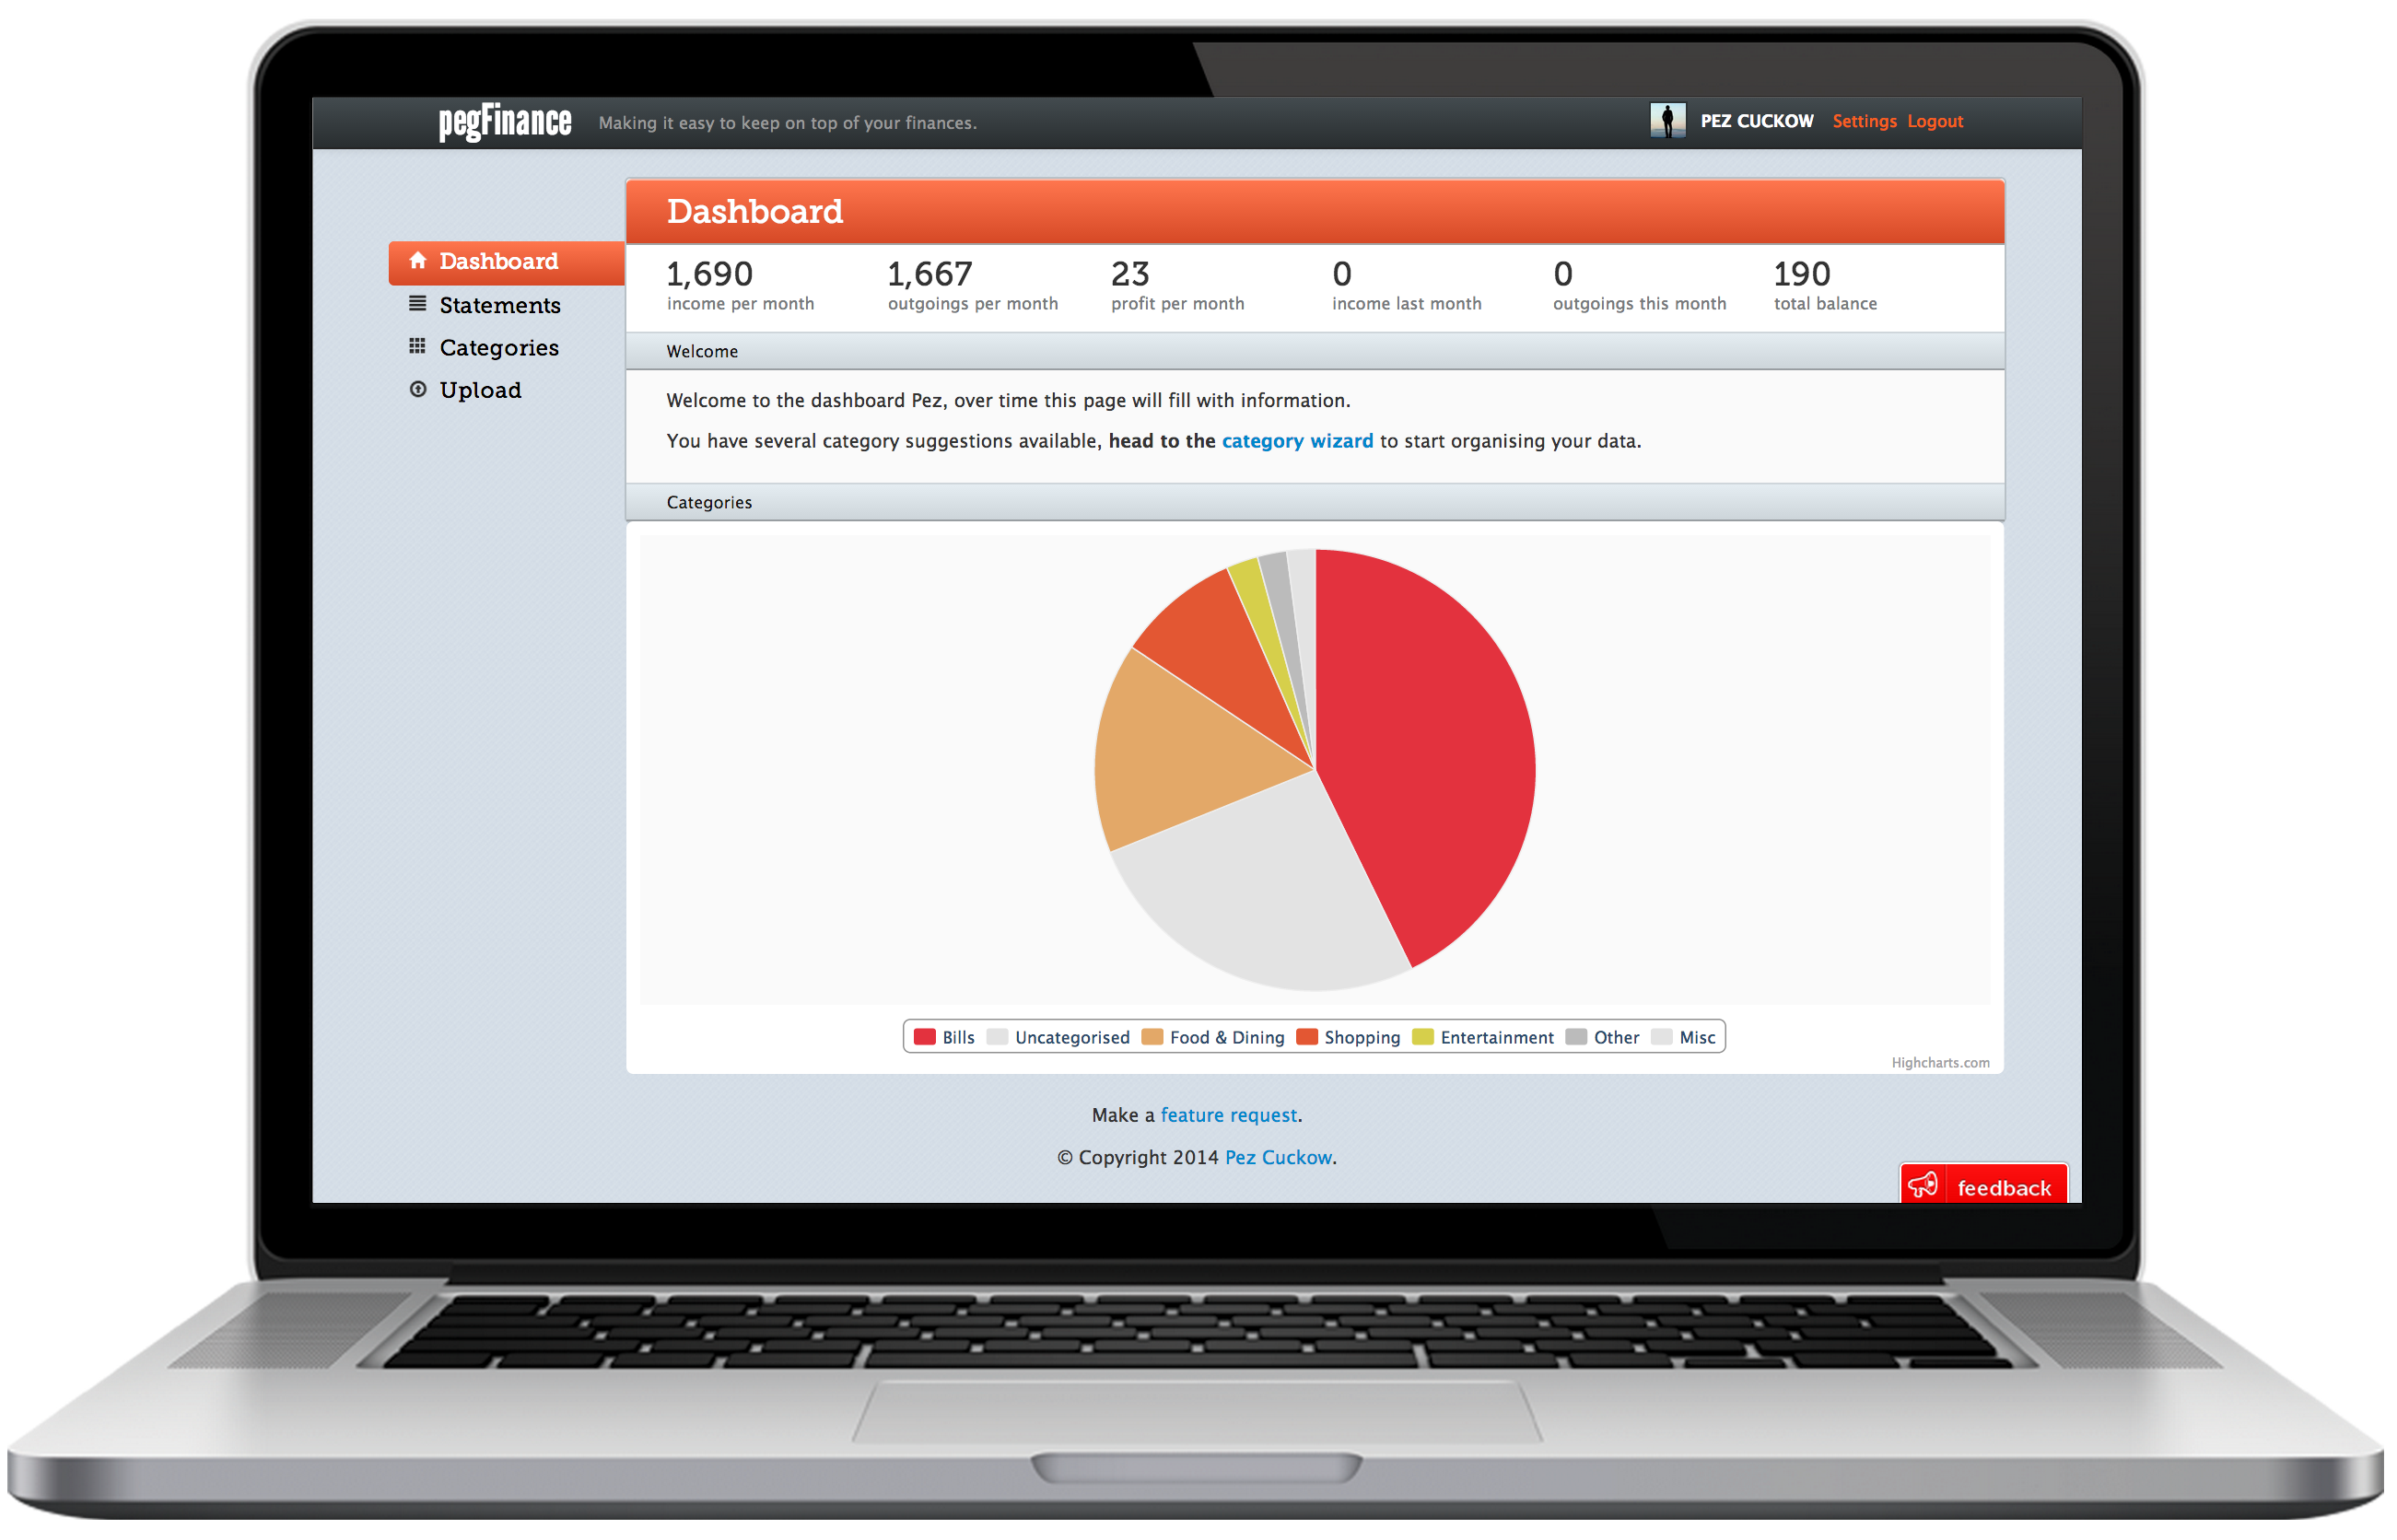
\includegraphics[width=0.8\textwidth]{screenshots/responsive/macbook}
    \caption{Layout on a standard laptop}
    \label{fig:responsive-macbook}
\end{figure}

\begin{figure}[h]
    \centering
    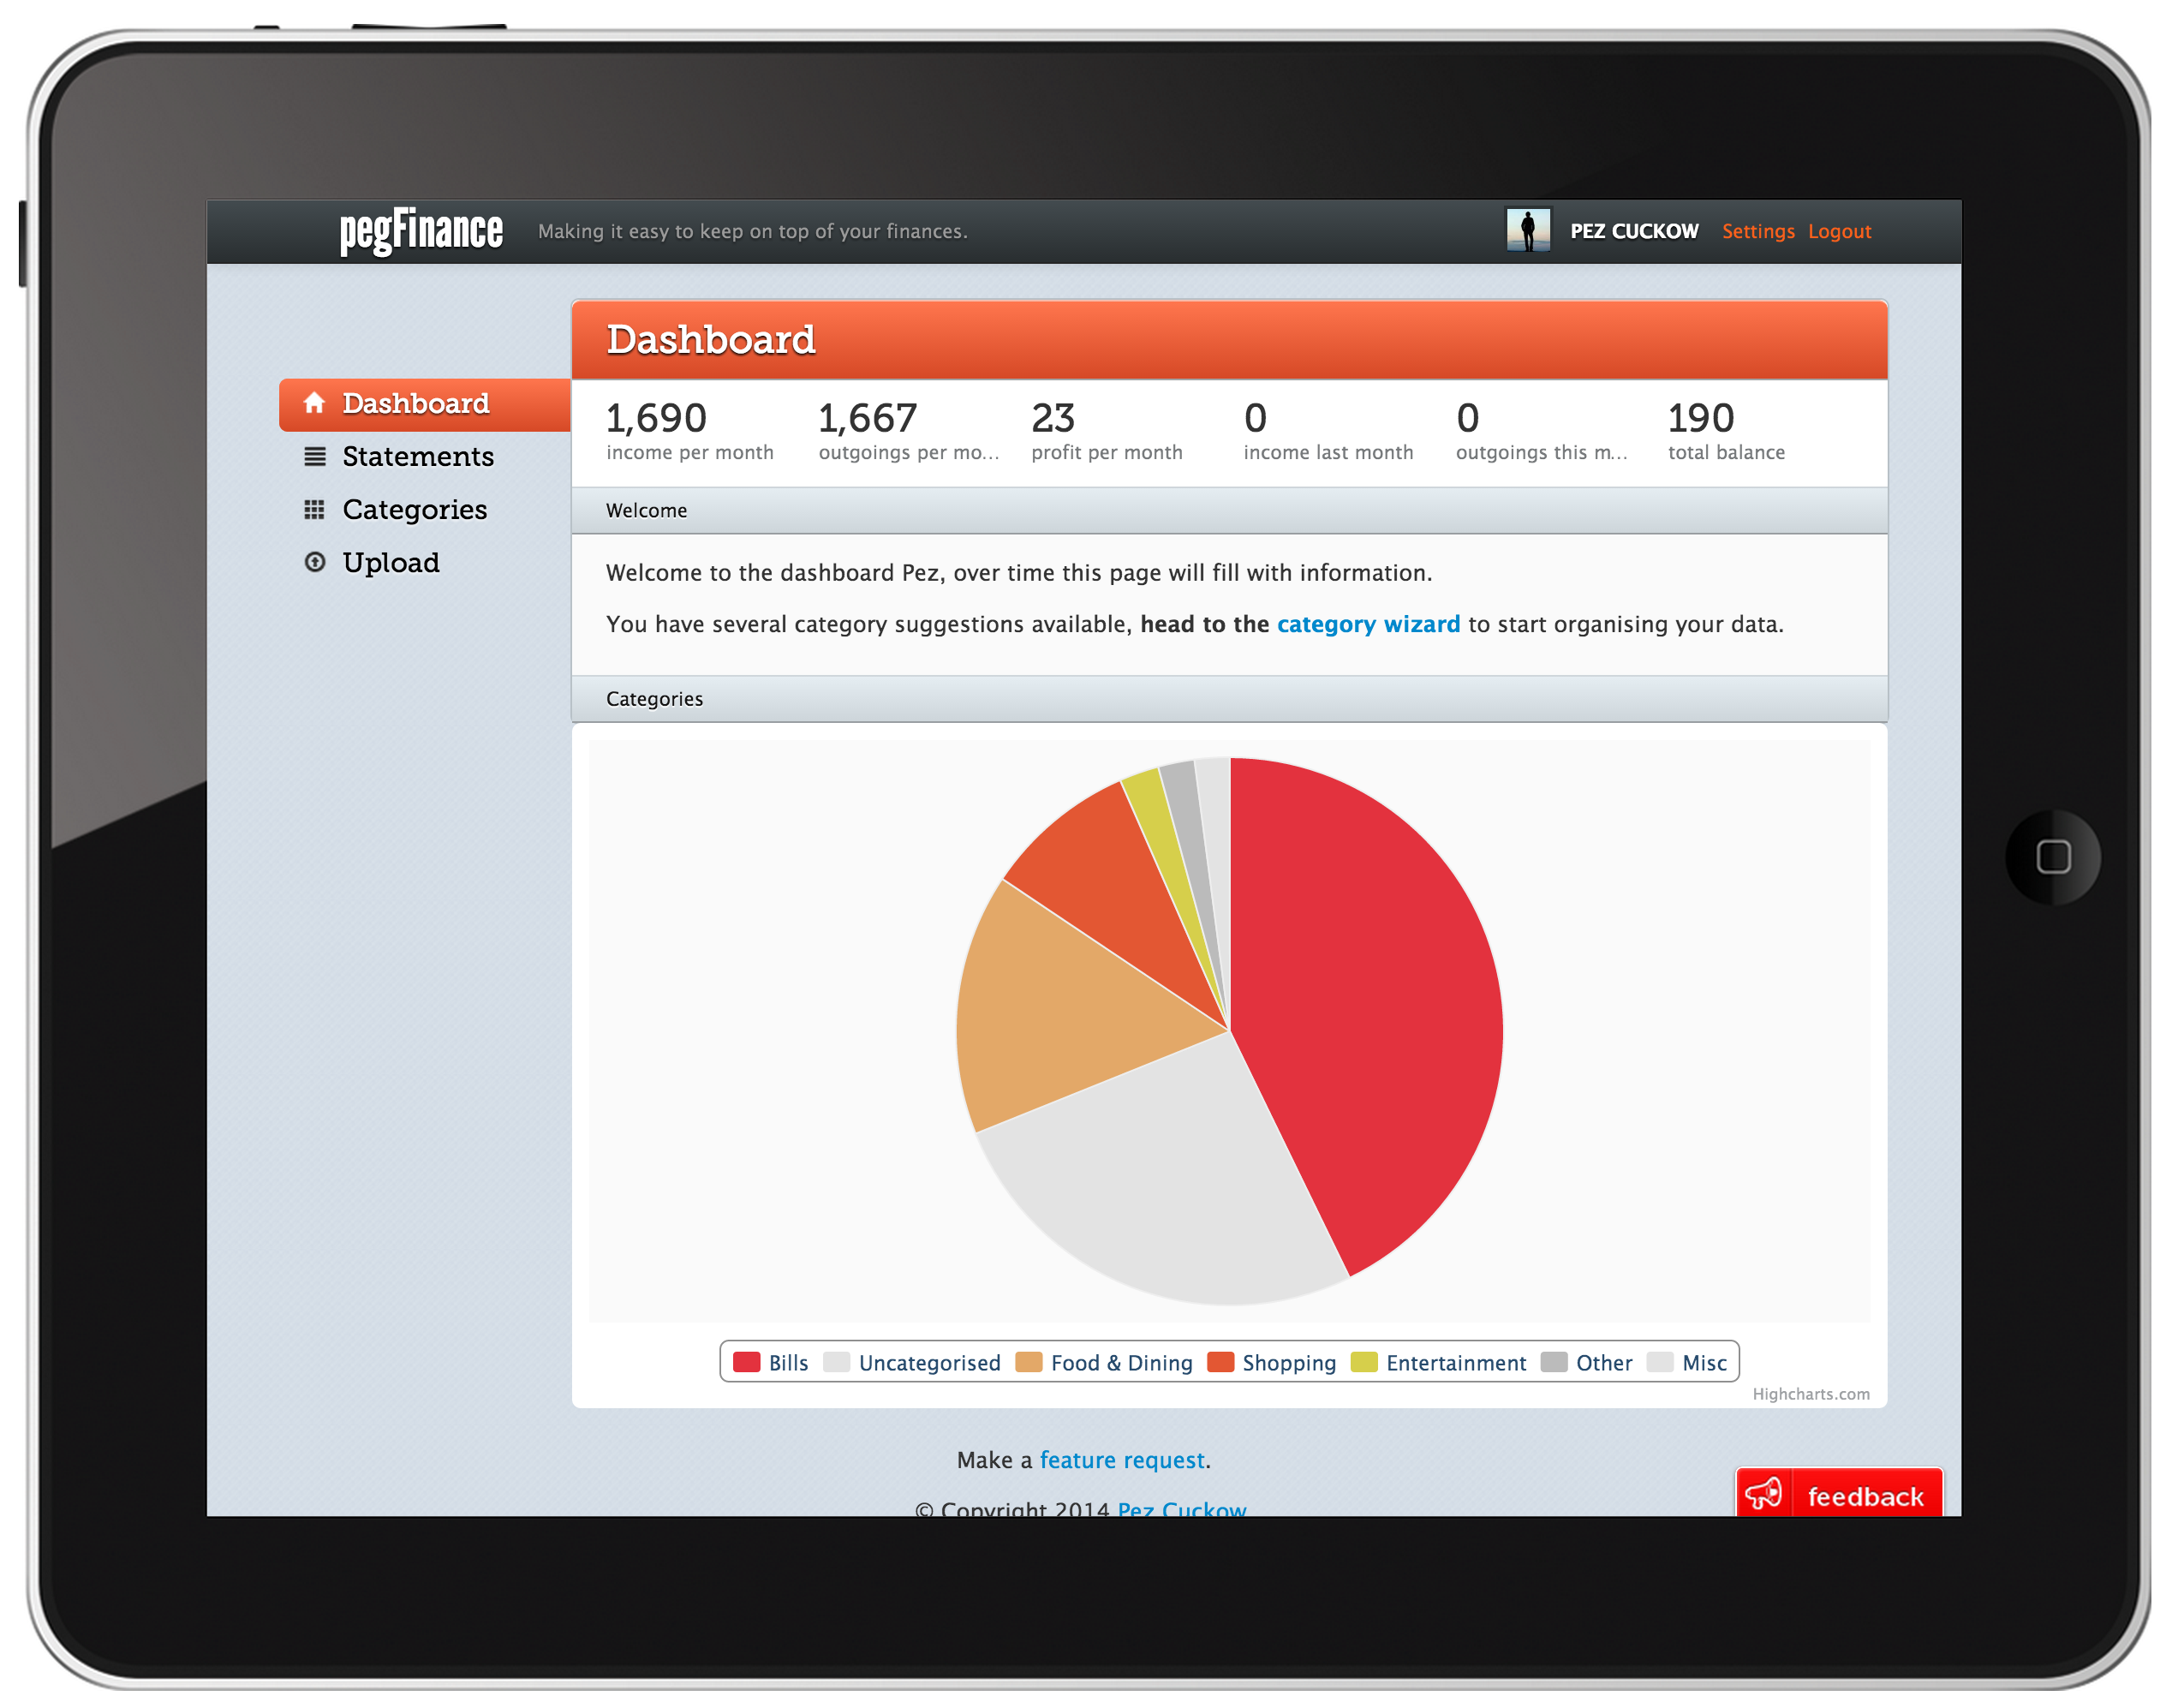
\includegraphics[width=0.8\textwidth]{screenshots/responsive/ipad-sideways}
    \caption{Layout on a tablet in landscape}
    \label{fig:responsive-ipad}
\end{figure}

\begin{figure}
\centering
\begin{minipage}{.5\textwidth}
    \centering
    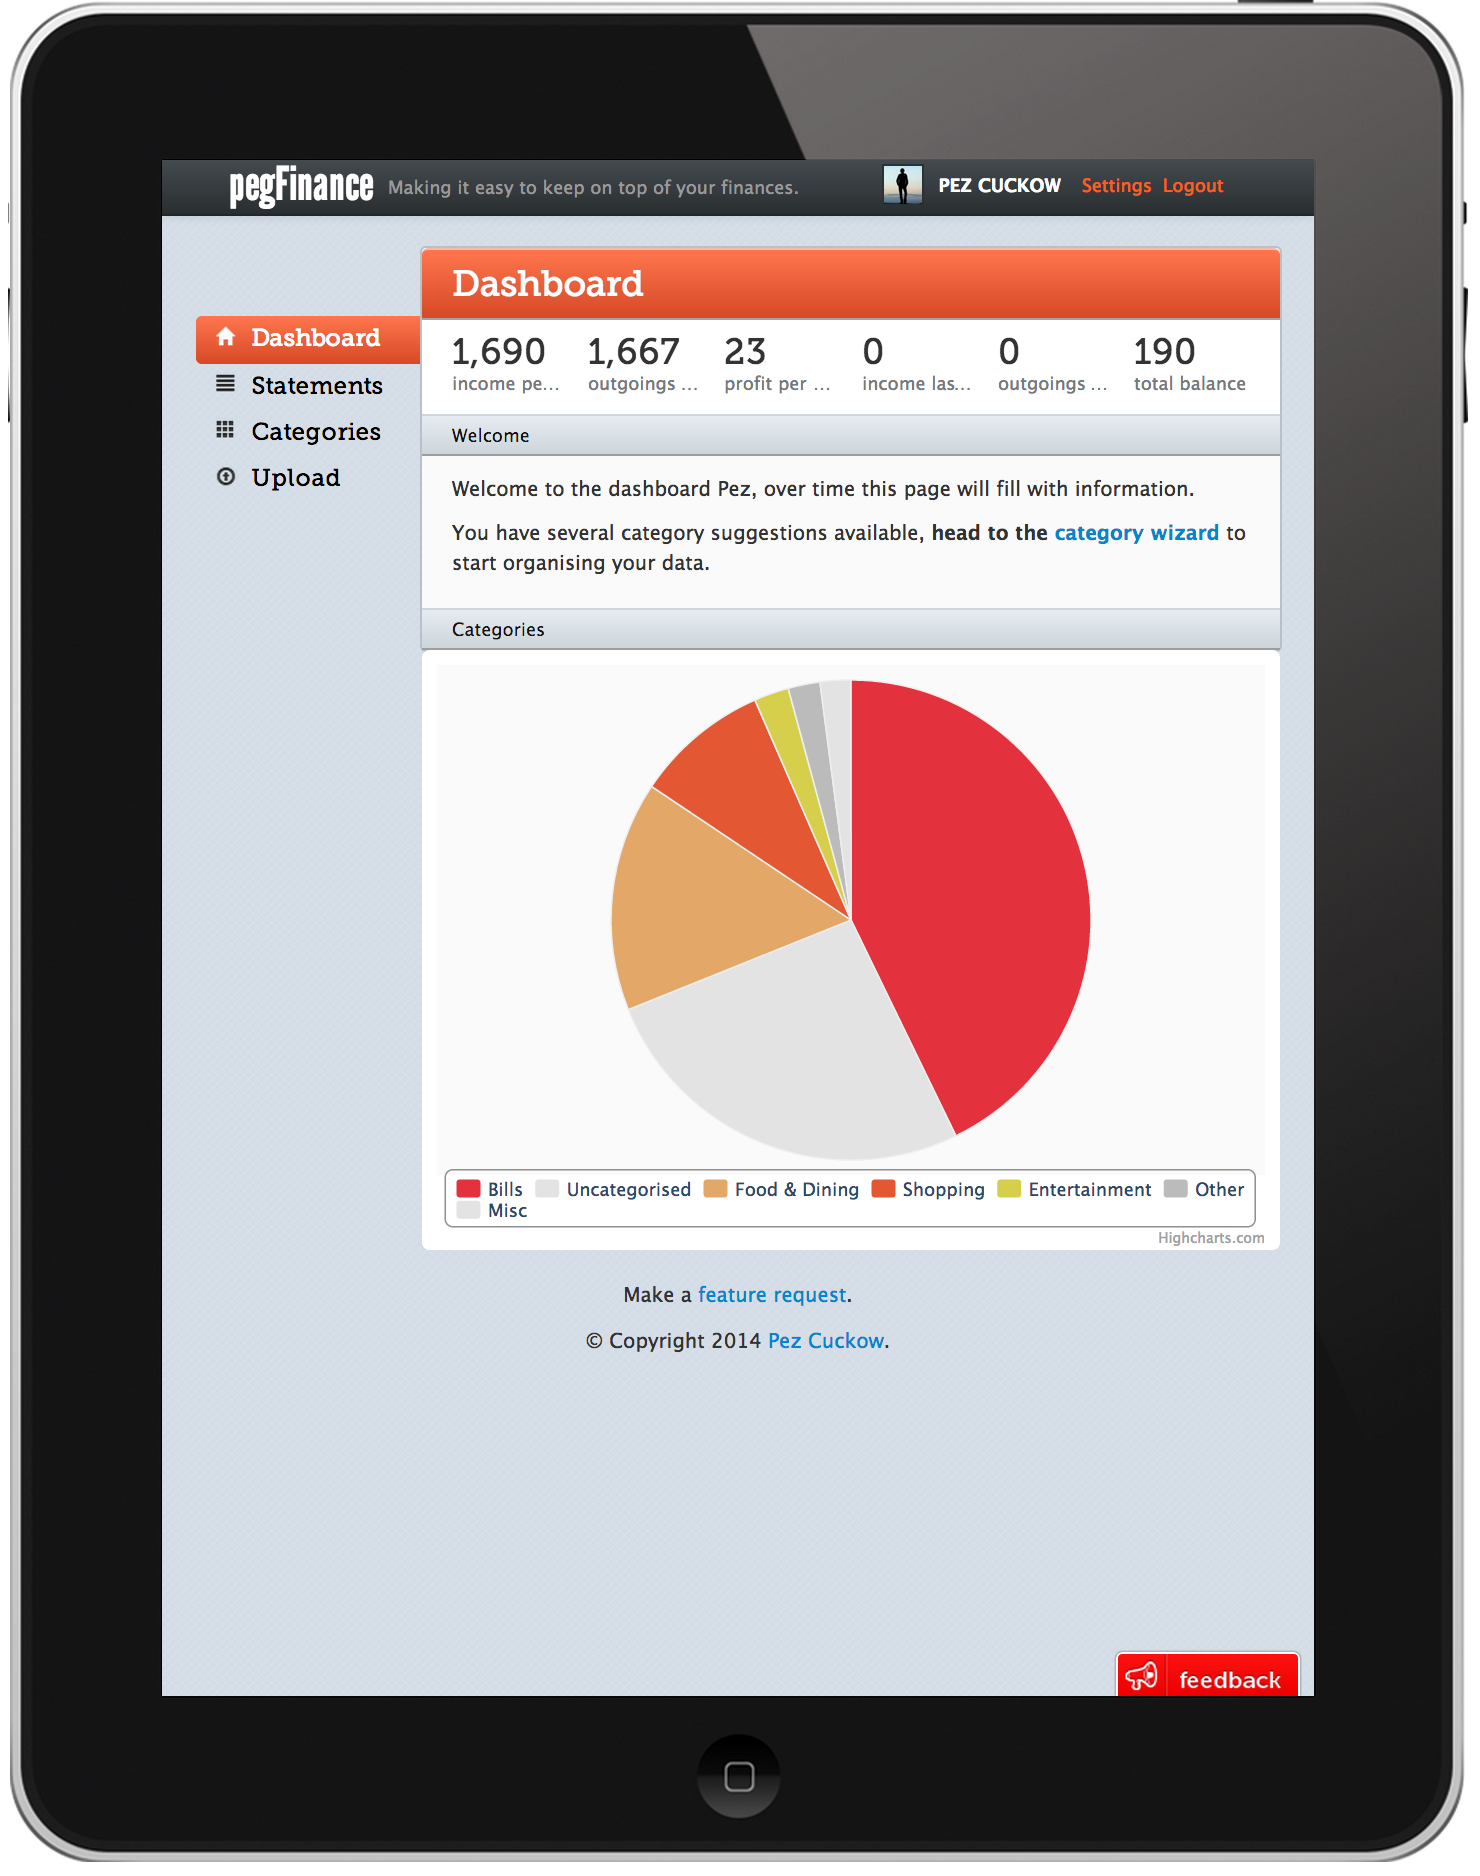
\includegraphics[width=0.45\textwidth]{screenshots/responsive/ipad-portrait}
    \captionof{figure}{Layout on a tablet in portrait}
    \label{fig:responsive-ipad2}
\end{minipage}%
\begin{minipage}{.5\textwidth}
    \centering
    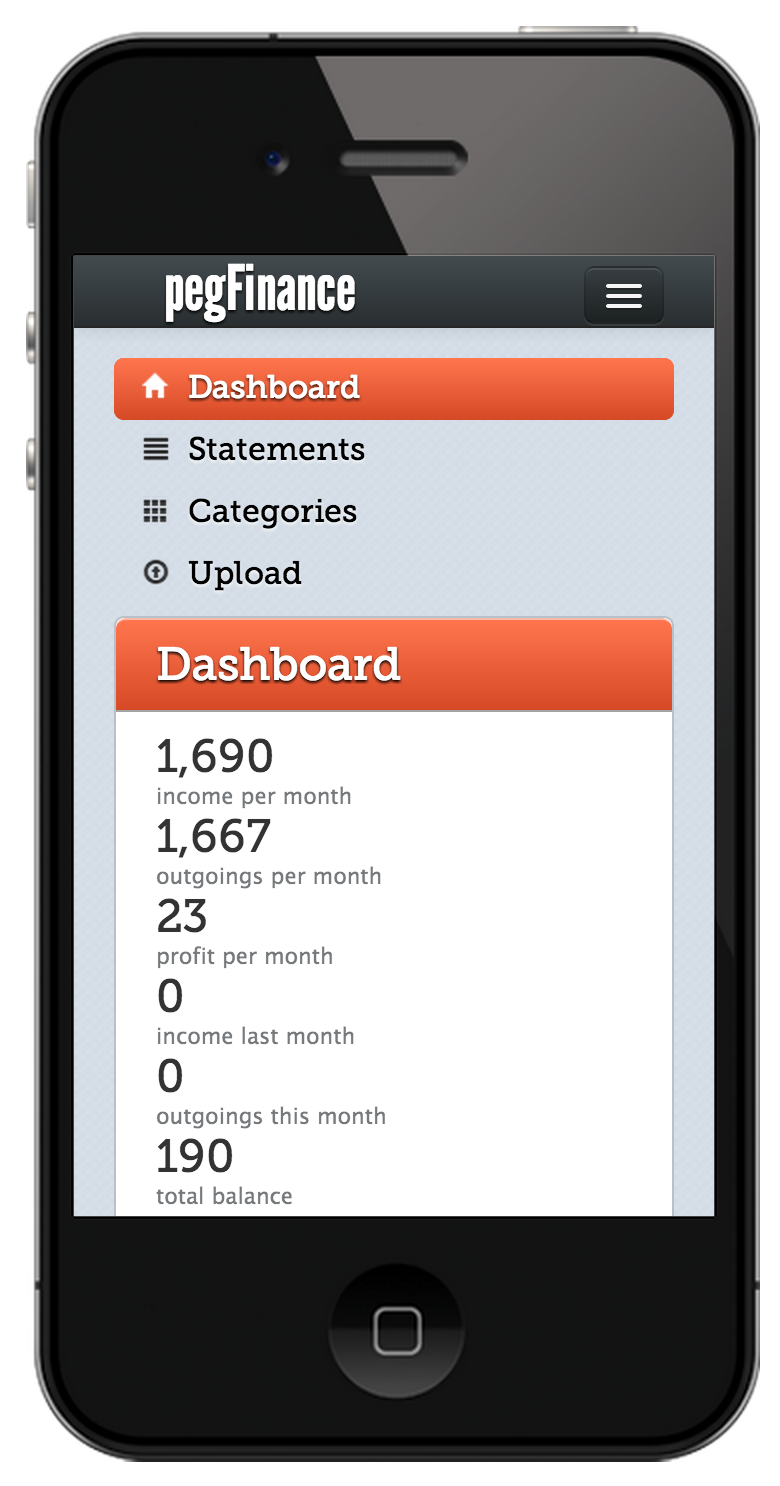
\includegraphics[width=0.5\textwidth]{screenshots/responsive/iphone-portrait}
    \captionof{figure}{Layout on a smaller smartphone}
    \label{fig:responsive-iphone}
\end{minipage}
\end{figure}

%\section{Uploading a Statement}

%\section{Suggestion Engine}

%\section{Viewing Statements}

%\section{Prediction Overview}